\documentclass[11pt,letterpaper]{article}

% ==================== PAQUETES ====================
\usepackage[utf8]{inputenc}
\usepackage[T1]{fontenc}
\usepackage[margin=2.5cm]{geometry}
\usepackage{mathptmx} % tipografía tipo Times New Roman (recomendada por APA)
\usepackage{titlesec}
\usepackage{fancyhdr}
\usepackage{tikz}
\usetikzlibrary{arrows.meta, positioning, fit, backgrounds}
\usepackage{booktabs}
\usepackage{array}
\usepackage{longtable}
\usepackage{caption}
\usepackage{enumitem}
\usepackage{needspace}
\usepackage{parskip}
\usepackage{pifont}
\usepackage{setspace}
\usepackage[hidelinks]{hyperref} % hidelinks = enlaces sin color, todo el texto en negro
\usepackage{xurl}

% ==================== ESTILO DE SECCIONES (todo en negro) ====================
\titleformat{\section}
  {\normalfont\Large\bfseries\color{black}}{\thesection}{0.6em}{}
\titleformat{\subsection}
  {\normalfont\large\bfseries\color{black}}{\thesubsection}{0.6em}{}
\titleformat{\subsubsection}
  {\normalfont\normalsize\bfseries\color{black}}{\thesubsubsection}{0.6em}{}

\pagestyle{fancy}
\fancyhf{}
\fancyhead[L]{\small\itshape IronVeil --- Framework de defensa en profundidad para LLMs autoalojados}
\fancyhead[R]{\small\itshape Fundamentos de Ciberseguridad}
\fancyfoot[C]{\thepage}
\renewcommand{\headrulewidth}{0.4pt}

\setlength{\parindent}{0pt}
\setlength{\parskip}{0.5em}

% ==================== NOMBRES EN ESPAÑOL (sin paquete babel-spanish) ====================
\renewcommand{\contentsname}{Índice}
\renewcommand{\abstractname}{Resumen}
\renewcommand{\figurename}{Figura}
\renewcommand{\tablename}{Tabla}

% ==================== COMANDO PARA REFERENCIAS APA ====================
% Entrada de bibliografía con sangría francesa (hanging indent), sin depender de bibtex/biber.
\newcommand{\refapa}[1]{%
  \par\noindent\hangindent=1.25cm\hangafter=1 #1\par\vspace{0.5em}%
}

% ==================== CITAS EN TEXTO CON HIPERVÍNCULO A LA REFERENCIA ====================
% \citeapa{clave}{texto mostrado} crea un enlace clicable hacia la entrada
% correspondiente en la sección de Referencias (marcada con \hypertarget{clave}{}).
\newcommand{\citeapa}[2]{\hyperlink{#1}{#2}}

% ==================== CAJAS DE NOTA (en blanco y negro) ====================
\newcommand{\notabox}[2]{%
\begin{center}
\fbox{%
\begin{minipage}{0.92\linewidth}
\vspace{3pt}
\small\textbf{#1:}\ #2
\vspace{3pt}
\end{minipage}%
}
\end{center}%
}

\begin{document}

% ======================================================================
% PORTADA (una sola hoja, formato APA)
% ======================================================================
\begin{titlepage}
\thispagestyle{empty}
\begin{center}

\vspace*{3.5cm}

{\Large\bfseries
IronVeil\par
\vspace{4pt}
{\large\normalfont Framework de Defensa en Profundidad Medible para LLMs Autoalojados\par}
\vspace{6pt}
\large\normalfont Evaluación Comparativa de Cinco Mecanismos Defensivos frente a los Vectores de Ataque\\
que ya Explotan 175\,000 Servidores Expuestos en Internet
\par}

\vspace{3.2cm}

{\large
Ana Gabriela Fiquitiva Poveda\par
Anderson Fabian García Nieto\par
Andrés Felipe Sabogal Wilches\par
Carlos Mario Piedrahita Arango
\par}

\vspace{3.2cm}

{\large
Escuela Colombiana de Ingeniería Julio Garavito\par
Fundamentos de Ciberseguridad\par
Profesor Diego Alexander López Correa\par
Octubre de 2026
\par
Bogota D.C., Colombia
\par}

\end{center}
\vspace*{\fill}
\end{titlepage}

\clearpage
\pagenumbering{arabic}

\begin{abstract}
\noindent
Miles de instancias del motor de inferencia local Ollama permanecen expuestas en internet sin autenticación, lo que en la práctica habilita a un atacante remoto a extraer \emph{system prompts} completos, desplazarse lateralmente entre modelos relacionados y agotar los recursos del servicio, sin necesidad de credenciales. La literatura reciente documenta que ninguna defensa aislada elimina este riesgo: técnicas de preprocesamiento de entradas alcanzan entre 60\,\% y 80\,\% de detección, mientras que arquitecturas más sofisticadas llegan hasta 95\,\% de protección contra patrones conocidos, pero conservan brechas relevantes frente a atacantes adaptativos. Este proyecto presenta \textbf{IronVeil}, un \emph{framework} de defensa en profundidad medible que despliega un laboratorio propio, aislado y controlado sobre Ollama, e implementa cinco mecanismos defensivos independientes y activables por separado (filtrado, delimitación de contenido, clasificación, mínimo privilegio y aprobación humana) para compararlos individualmente y en combinación frente a una batería reproducible de cinco vectores de ataque documentados en la industria y en la academia. A diferencia de las soluciones comerciales que dominan el mercado actual (Prisma AIRS de Palo Alto Networks, FortiAIGate de Fortinet, Lakera Guard de Check Point), orientadas a proteger modelos alojados en servicios cloud gestionados, IronVeil se enfoca deliberadamente en el punto ciego de los despliegues autoalojados y aporta evidencia empírica comparativa --inexistente hoy en el mercado-- sobre qué combinación de mecanismos ofrece la mejor relación entre protección, latencia añadida, falsos positivos y costo de implementación. Este documento actualiza la propuesta inicial con lo implementado y medido: sobre cinco corridas en GPU T4 con \texttt{llama3.2:1b}, el ASR promedio de los vectores 1 a 4 baja de 31,2\,\% en el \emph{baseline} a 15,0\,\% con filtrado solo y con los cinco mecanismos; filtrado, delimitación y mínimo privilegio muestran efecto medible con un costo de latencia inferior a 1\,ms, la clasificación añade cerca de 76\,ms sin una reducción de fuga distinguible con este modelo, y ninguna configuración llega a 0\,\%. Como extensiones medidas aparte del núcleo, el trabajo evalúa un clasificador alternativo de pago (Jev, de TypeSafe) frente al clasificador local Llama Prompt Guard 2: en la validación externa con Garak (339 ataques), el clasificador Jev solo dejó pasar 1 de 339 ataques (0,3\,\%) y, combinado con el resto de mecanismos del proxy, 0 de 339 (intervalo de confianza del 95\,\% de 0,0\,\% a 1,1\,\%), frente a 51,2\,\% sin defensas; se documenta además la comparación de latencia, cobertura de idiomas y costo (punto de equilibrio de unos 17 millones de peticiones al mes bajo los supuestos declarados). El proxy se distribuye como \emph{framework}: laboratorio completo con un solo comando de Docker Compose, paquete instalable (\texttt{pip install ironveil}) y autenticación opcional.

\vspace{0.5em}
\noindent\textbf{Palabras clave:} seguridad en modelos de lenguaje, \emph{prompt injection}, defensa en profundidad, Ollama, OWASP LLM Top 10, \emph{guardrails}, mínimo privilegio, aprobación humana, AI-SPM, SIEM, Jev, Llama Prompt Guard, Garak.
\end{abstract}

\clearpage

\tableofcontents
\clearpage

% ======================================================================
\section{Introducción y Estado del Arte}
% ======================================================================

\subsection{El problema: instancias LLM autoalojadas expuestas en internet}

Ollama fue diseñado como una herramienta de uso local y, por esa razón, no incorpora autenticación por defecto. Cuando un equipo de desarrollo configura la variable de entorno \texttt{OLLAMA\_HOST=0.0.0.0} para permitir el acceso desde otra máquina (algo común en despliegues en la nube o en contenedores), el servicio queda expuesto a cualquier persona en internet sin ninguna barrera de entrada.

La magnitud del problema ha crecido de forma sostenida y bien documentada. Una investigación conjunta de SentinelLabs (SentinelOne) y Censys, que analizó 7{,}23 millones de observaciones a lo largo de 293 días, identificó 175\,108 servidores Ollama únicos (aproximadamente 175\,000) expuestos públicamente en 130 países y 4\,032 sistemas autónomos, con una porción persistente de alrededor de 23\,000 hosts responsables de la mayor parte de la actividad observada \citeapa{sentinelone2026}{(SentinelOne, 2026)}. Un hallazgo especialmente relevante para justificar este proyecto es que cerca de la mitad de esos servidores (más del 48\,\%) anuncian la funcionalidad de \emph{tool calling} en su API, es decir, no son simples fugas pasivas de información sino puntos de entrada activos capaces de ejecutar código e interactuar con sistemas externos \citeapa{sentinelone2026}{(SentinelOne, 2026)}.

En mayo de 2026, investigadores de Cyera divulgaron una vulnerabilidad crítica en Ollama denominada \emph{Bleeding Llama} (CVE-2026-7482, CVSS 9.1): una lectura fuera de límites en el cargador de archivos GGUF que permite a un atacante no autenticado filtrar memoria del \emph{heap} del proceso (claves de API, variables de entorno, \emph{system prompts} y conversaciones de otros usuarios) mediante tres llamadas a la API. Cyera estimó que la vulnerabilidad afectaba a cerca de 300\,000 servidores expuestos a nivel global \citeapa{cyera2026}{(Cyera Research, 2026)}; las versiones anteriores a la 0.17.1 son las vulnerables \citeapa{thn2026}{(The Hacker News, 2026)}. Este hallazgo confirma, con un caso concreto y reciente, el patrón de riesgo que motiva el proyecto: exposición sin autenticación, fuga de \emph{system prompt} y credenciales, y superficie de ataque que crece junto con la adopción de la herramienta.

\subsection{Marco de riesgo: OWASP Top 10 para aplicaciones LLM (2025)}

La referencia estándar de la industria para clasificar riesgos de seguridad en sistemas basados en LLM es el \emph{OWASP Top 10 for LLM Applications}, publicado por el OWASP GenAI Security Project y actualizado en su edición 2025 \citeapa{owasp2025}{(OWASP GenAI Security Project, 2025)}. \emph{Prompt Injection} (LLM01) mantiene el primer lugar por segunda edición consecutiva: dado que los LLM procesan instrucciones y datos por el mismo canal sin una separación estructural clara, un atacante puede construir una entrada que el modelo interprete como una instrucción nueva en lugar de como contenido a procesar. La edición 2025 también reordenó \emph{Sensitive Information Disclosure} (LLM02) al segundo lugar, incorporó \emph{System Prompt Leakage} (LLM07) como categoría nueva (tras incidentes reales donde se extrajeron las reglas internas y la lógica de filtrado de sistemas en producción) y amplió \emph{Excessive Agency} (LLM06) para cubrir los riesgos de agentes con herramientas y permisos excesivos. Este proyecto se alinea directamente con LLM01, LLM02, LLM06, LLM07 y LLM10 (\emph{Unbounded Consumption}); dentro del alcance quedan explícitamente fuera LLM03 (\emph{Supply Chain}), LLM04 (\emph{Data and Model Poisoning}), LLM08 (\emph{Vector and Embedding Weaknesses}, propio de sistemas RAG) y LLM09 (\emph{Misinformation}), por las razones que se detallan en la sección de Alcance.

\subsection{Evidencia académica sobre la eficacia de las defensas}

La pregunta que sostiene este proyecto (qué combinación de mecanismos ofrece mejor protección con menor impacto en utilidad y costo) está directamente respaldada por la literatura académica reciente. Una revisión sistemática que sintetiza 128 estudios revisados por pares entre 2022 y 2025, siguiendo las directrices de Kitchenham, encontró que las técnicas de ataque evolucionaron rápidamente de inyecciones directas simples a ataques multimodales sofisticados, logrando tasas de éxito superiores al 90\,\% contra sistemas sin ninguna protección. La misma revisión reporta que el preprocesamiento de entradas (una defensa relativamente simple, análoga al mecanismo de \emph{filtrado} de este proyecto) logra entre 60\,\% y 80\,\% de tasa de detección, mientras que las defensas arquitectónicas más avanzadas alcanzan hasta 95\,\% de protección contra patrones de ataque conocidos, pero persisten brechas importantes contra ataques nuevos o adaptativos \citeapa{geng2026}{(Geng, Xu, Qu \& Wong, 2026)}. Esta misma fuente identifica 37 enfoques de defensa distintos agrupados en tres niveles (preprocesamiento de entrada, arquitectura de sistema y nivel de modelo) que corresponden, de forma natural, a los cinco mecanismos que este proyecto aísla y mide por separado.

En la práctica de la industria, Microsoft documenta una estrategia de defensa en profundidad contra la inyección indirecta de \emph{prompts} que combina tres capas: prevención mediante la técnica de \emph{Spotlighting} (marcado estructural del texto no confiable mediante delimitación, marcado de datos o codificación, para que el modelo distinga instrucciones de datos), detección mediante un clasificador (\emph{Prompt Shields}) y salvaguardas deterministas que limitan el impacto incluso cuando la inyección tiene éxito \citeapa{microsoft2025}{(Microsoft Security Response Center, 2025)}. La técnica de \emph{Spotlighting} fue propuesta originalmente por \citeapa{hines2024}{Hines et al. (2024)} y corresponde directamente al mecanismo de \emph{delimitación de contenido} de este proyecto. En la misma línea, trabajos académicos como StruQ \citeapa{struq2025}{(Chen, Piet, Sitawarin \& Wagner, 2025)} y SecAlign \citeapa{secalign2025}{(Chen et al., 2025)} proponen aplicar el principio de \emph{separación de control y datos}, propio de la seguridad de software tradicional, directamente en la arquitectura del LLM.

Sobre el mecanismo de mínimo privilegio, Unit 42, el equipo de inteligencia de amenazas de Palo Alto Networks, recomienda explícitamente limitar a los agentes de IA al mínimo de herramientas y permisos necesarios, y exigir una capa adicional de aprobación humana para las acciones de alto impacto, señalando que ``no existe una forma determinista de proteger a los agentes de realizar acciones maliciosas'' salvo reducir sus permisos al mínimo indispensable \citeapa{unit42a2026}{(Unit 42, Palo Alto Networks, 2026a)}. El mismo equipo advierte que los \emph{guardrails} de contenido son una defensa ``blanda'' (detectan y bloquean la mayoría de los intentos, pero es actualmente imposible bloquear de forma determinista el cien por ciento de los ataques), mientras que reducir permisos es una defensa ``dura'' y determinista \citeapa{unit42b2026}{(Unit 42, Palo Alto Networks, 2026b)}. Esta distinción entre defensas probabilísticas (filtrado, clasificación) y defensas estructurales (delimitación, mínimo privilegio) es central en el diseño de este proyecto y coincide con la conclusión de la revisión de \citeapa{geng2026}{Geng et al. (2026)}: ninguna defensa aislada es suficiente, por lo que la pregunta relevante no es cuál mecanismo es mejor, sino qué combinación ofrece la mejor relación entre protección, latencia y usabilidad.

\subsection{Herramientas de la industria: ataque y defensa}

Del lado ofensivo, las principales herramientas open-source usadas para evaluar sistemáticamente estas vulnerabilidades son Garak (NVIDIA), orientado al escaneo amplio de un modelo con más de 120 pruebas (\emph{probes}); PyRIT (Microsoft), especializado en ataques multiturno con escalamiento conversacional (\emph{crescendo}); y Promptfoo, que permite automatizar pruebas dentro de un pipeline de integración continua. Del lado defensivo, NeMo Guardrails (NVIDIA) es un \emph{framework} de ``rieles'' de conversación programables que controla el flujo completo del diálogo, y frecuentemente utiliza Llama Guard (Meta), un modelo clasificador de seguridad de contenido, como el componente que ejecuta la validación semántica por debajo. Ambas herramientas no son competidoras sino piezas complementarias, lo cual respalda directamente la premisa de IronVeil: ningún componente cubre por sí solo todas las capas del problema, y la mayoría de sistemas en producción combinan dos o más.

\subsection{Panorama de mercado y diferenciación competitiva}
\label{sec:mercado}

Antes de presentar la propuesta, es necesario responder una pregunta que cualquier evaluador con criterio de mercado formulará de inmediato: ¿ya existen productos comerciales para este problema, y en qué se diferencia IronVeil de ellos?

\textbf{El mercado se está consolidando por adquisiciones, no por consenso técnico.} En los últimos dieciocho meses, los grandes proveedores de ciberseguridad compraron a las startups especializadas en seguridad de IA en lugar de construir esta capacidad desde cero: Palo Alto Networks adquirió Protect AI (julio de 2025) y lanzó \emph{Prisma AIRS}, que cubre escaneo de modelos, seguridad de la cadena de suministro, \emph{red teaming} automatizado y protección en tiempo de ejecución \citeapa{getmaxim2026}{(Maxim AI, 2026)}; Check Point adquirió Lakera, cuyo producto Lakera Guard clasifica \emph{prompts} y respuestas en tiempo real con más de 98\,\% de tasa de detección y menos de 50\,ms de latencia \citeapa{wiz2026}{(Wiz, 2026)}; Cisco adquirió Robust Intelligence; y SentinelOne adquirió Prompt Security. Fortinet, por su parte, no adquirió sino que desarrolló internamente \emph{FortiAIGate}, un \emph{gateway} de seguridad en tiempo de ejecución que se sitúa entre la aplicación y el modelo, aplica \emph{guardrails} sobre la entrada y la salida, y mapea su cobertura explícitamente contra el OWASP Top 10 para LLM \citeapa{fortinet2026}{(Fortinet, 2026)}.

Un dato relevante para contextualizar la madurez de esta categoría: a la fecha de este documento \textbf{no existe un Cuadrante Mágico de Gartner dedicado específicamente a ``seguridad de LLM''} como categoría independiente; un análisis de mercado de abril de 2026 confirma explícitamente que la categoría adyacente de ``AI SOC'' tampoco cuenta todavía con Cuadrante Mágico ni con Forrester Wave propios \citeapa{securityboulevard2026}{(Security Boulevard, 2026)}. Esto no significa que el mercado esté vacío --como muestra la lista de adquisiciones anterior, está lejos de estarlo-- sino que es una categoría emergente sin un estándar de evaluación consolidado, exactamente el tipo de espacio donde un aporte empírico y comparativo como el de IronVeil tiene valor diferencial.

\begin{center}
\small
\begin{tabular}{@{}p{3.0cm}p{5.6cm}p{5.4cm}@{}}
\toprule
\textbf{Herramienta} & \textbf{Qué SÍ resuelve} & \textbf{Qué NO cubre (brecha frente a IronVeil)} \\
\midrule
Lakera Guard (Check Point) & Clasifica \emph{prompts}/respuestas en tiempo real; funciona con \emph{backends} autoalojados \citeapa{wiz2026}{(Wiz, 2026)} & Caja negra comercial de pago; no combina 5 mecanismos medibles por separado ni publica evidencia comparativa de qué combinación protege mejor \\
Prisma AIRS (Palo Alto, ex-Protect AI) & Cubre todo el ciclo de vida: escaneo de modelos, \emph{supply chain}, \emph{red teaming} automático, \emph{runtime} \citeapa{getmaxim2026}{(Maxim AI, 2026)} & Orientado a grandes empresas ya licenciadas en el ecosistema Palo Alto; no aísla el efecto individual de cada mecanismo \\
FortiAIGate (Fortinet) & \emph{Gateway} empresarial con \emph{guardrails}, límite de tasa y mitigación de DDoS, mapeado al OWASP Top 10 LLM \citeapa{fortinet2026}{(Fortinet, 2026)} & Requiere aceleración por hardware (SmartNIC/GPU) y licenciamiento FortiCare; inviable para un laboratorio autoalojado pequeño; no publica comparativas por capa \\
HiddenLayer & Protege el modelo mismo: detección de robo, \emph{tampering} y manipulación de pesos \citeapa{checkpoint2026}{(Check Point Software, 2026)} & No ataca el vector conversacional (inyección de \emph{prompt} vía texto), que es el núcleo de IronVeil \\
Guías de \emph{hardening} manual (nginx + auth + firewall) & Es la práctica más documentada hoy para exponer Ollama de forma menos insegura \citeapa{aithinkerlab2026}{(AI Thinker Lab, 2026)} & Cubren solo el control de acceso perimetral; ningún tutorial mide ni compara el efecto de capas adicionales \\
llm-shield (proyecto independiente en GitHub) & \emph{Gateway} + \emph{firewall} + monitoreo específico para IA autoalojada, en fase temprana de desarrollo \citeapa{githubllmshield2026}{(JTHil, 2026)} & Producto individual de un desarrollador; no implementa mínimo privilegio entre modelos ni aprobación humana, ni evaluación comparativa empírica \\
\bottomrule
\end{tabular}
\end{center}

\notabox{¿Ya existen ``plugins'' de solo integrar y listo?}{Sí, para un mecanismo aislado: la clasificación de contenido. Lakera Guard, por ejemplo, es literalmente una API que se integra en pocas líneas de código \citeapa{wiz2026}{(Wiz, 2026)}. Pero ningún producto comercial ni de código abierto combina los cinco mecanismos con mínimo privilegio entre modelos autoalojados relacionados y aprobación humana como capas independientes y medibles por separado, y sobre todo, ninguno publica evidencia empírica comparativa de qué combinación ofrece la mejor relación protección/utilidad/costo. Los proveedores venden su propia solución como la mejor; IronVeil mide, con datos propios, si eso es cierto y bajo qué condiciones.}

Finalmente, es importante precisar el terreno específico donde compite IronVeil. La inmensa mayoría de las herramientas comerciales listadas arriba --incluyendo Prisma AIRS, FortiAIGate y los \emph{guardrails} nativos de AWS Bedrock y Azure AI Content Safety-- están diseñadas para proteger \textbf{modelos alojados en servicios cloud gestionados por el propio proveedor}. El problema que motiva este proyecto (Sección~1.1) --175\,000 instancias Ollama expuestas, con 48\,\% permitiendo ejecución de código \citeapa{sentinelone2026}{(SentinelOne, 2026)}-- es precisamente el punto ciego que esas herramientas de nube gestionada no cubren, porque el modelo no vive en su infraestructura. IronVeil no compite por el mismo mercado que Prisma AIRS o FortiAIGate: ataca el nicho específico, real y creciente, de los despliegues autoalojados sin gestión centralizada.

% ======================================================================
\section{Problema que se Abordará}
% ======================================================================

Miles de instancias de LLM autoalojados, con Ollama como caso representativo y ampliamente documentado, se exponen accidentalmente en internet sin autenticación, principalmente por errores de configuración durante el despliegue. Esto permite a un atacante extraer \emph{system prompts} completos, realizar movimiento lateral entre modelos relacionados dentro de la misma organización, y agotar los recursos del servicio, todo ello sin necesidad de credenciales válidas.

El problema no es únicamente la ausencia de protección: es que, en la práctica, las organizaciones suelen implementar un único mecanismo de defensa de forma aislada (por ejemplo, solo un filtro de palabras, o solo autenticación de red) sin evidencia clara de qué combinación de los mecanismos disponibles reduce realmente el riesgo sin volver el sistema inutilizable o costoso de mantener. La literatura académica reciente confirma esta brecha: existen decenas de mecanismos de defensa propuestos de forma individual, pero pocos estudios comparan sistemáticamente combinaciones de mecanismos heterogéneos (basados en reglas, en clasificadores, en control de acceso y en supervisión humana) sobre un mismo sistema y con la misma batería de ataques.

Existe, además, una brecha operativa que rara vez se documenta junto con la brecha técnica anterior: incluso cuando un mecanismo de defensa bloquea correctamente un ataque, ese bloqueo suele quedar silencioso. Sin un canal de notificación, el equipo de seguridad no se entera del incidente en el momento en que ocurre; y sin una integración con un sistema de gestión de eventos e información de seguridad (SIEM), ese evento tampoco puede correlacionarse con el resto de la actividad de seguridad de la organización. Una defensa técnicamente efectiva pero operativamente invisible no cierra el ciclo completo de detección y respuesta. Este proyecto aborda también esa brecha mediante una extensión ya implementada: exportación del mismo \emph{log} que generan los cinco mecanismos en formatos JSON, CEF, LEEF y ECS hacia un SIEM (con reglas de Wazuh incluidas) y avisos por \emph{webhook}, Slack o correo cuando la aprobación humana encola una petición (Sección~6).

% ======================================================================
\section{Pregunta y Objetivos de Investigación}
% ======================================================================

\subsection{Pregunta de investigación}

{¿Qué combinación de los cinco mecanismos defensivos (filtrado, delimitación de contenido, clasificación, mínimo privilegio y aprobación humana) reduce de forma más efectiva la tasa de éxito de los vectores de ataque documentados contra LLM autoalojados, con el menor impacto posible en utilidad y costo de implementación?}

\subsection{Objetivo general}

Evaluar comparativamente, a través de \textbf{IronVeil}, los cinco mecanismos defensivos definidos, individualmente y en combinación, mediante la ejecución sistemática de una batería de ataques reproducibles, para determinar la combinación con mejor relación protección/utilidad/costo.

\subsection{Objetivos específicos}

\begin{enumerate}[leftmargin=1.4cm, itemsep=2pt]
\item Caracterizar el estado actual del problema de exposición de LLM autoalojados en internet, con base en literatura técnica y académica reciente.
\item Diseñar y desplegar un laboratorio controlado que replique el patrón de vulnerabilidad documentado en instancias reales de Ollama.
\item Implementar los cinco mecanismos defensivos como módulos independientes, activables y desactivables sobre un mismo \emph{pipeline}.
\item Ejecutar una batería reproducible de cinco vectores de ataque contra el \emph{baseline}, contra cada mecanismo por separado y contra la combinación completa.
\item Medir y comparar tasa de éxito de ataque, latencia añadida, falsos positivos y costo de implementación por mecanismo y por combinación.
\item Formular una recomendación basada en evidencia sobre la combinación de mecanismos más efectiva para este contexto.
\item Como extensión (implementada y fuera de las siete configuraciones del núcleo), cerrar el ciclo de detección-respuesta mediante notificación al usuario ante bloqueos de riesgo y una integración con un SIEM que centralice y correlacione los eventos generados por los cinco mecanismos.
\end{enumerate}

% ======================================================================
\section{Alcance}
% ======================================================================

\subsection{Dentro del alcance}

\begin{itemize}[leftmargin=1.2cm]
\item Un laboratorio propio, aislado y autorizado (contenedores Docker, red interna cerrada). En ningún momento se atacan instancias reales de terceros expuestas en internet.
\item Ollama como plataforma de estudio, con dos modelos (\texttt{soporte} y \texttt{rrhh}) basados en \texttt{llama3.2} (versión de 1B en las corridas de Colab con GPU T4 y de 3B en la demo local) que simulan distintos ``departamentos'' con información sensible ficticia plantada a propósito.
\item Un único \emph{pipeline} (proxy en Python) situado entre el cliente y Ollama, con los cinco mecanismos implementados como módulos independientes, activables y desactivables mediante un archivo de configuración.
\item Siete configuraciones de prueba: \emph{baseline} (todos los mecanismos apagados), cada mecanismo activado individualmente (cinco configuraciones) y la combinación completa de los cinco. Si el cronograma lo permite, se explorarán combinaciones parciales adicionales (por ejemplo, filtrado + clasificación) para enriquecer el análisis de costo/beneficio.
\item Cinco vectores de ataque núcleo: reconocimiento de servicio, extracción de \emph{system prompt}, inyección de \emph{prompts} (directa e indirecta vía conversación), movimiento lateral (simulado con credenciales ficticias plantadas) y agotamiento de recursos.
\item Automatización de las pruebas con herramientas estándar de la industria (Garak y Promptfoo) e integración continua en GitHub Actions (formato, análisis estático y pruebas unitarias sin necesidad de levantar Docker ni Ollama).
\item Extensiones opcionales, apagadas por defecto y registradas aparte del núcleo (sus filas llevan una marca de extensión y las tablas del núcleo las excluyen): un escenario de \emph{Excessive Agency} (V7) con herramientas simuladas en el modelo \texttt{rrhh-agente}; validación externa con Garak sobre una segunda instancia del proxy; normalización de entrada (decodificación de Base64, hexadecimal, ROT13 y caracteres invisibles antes de la cadena); memoria de decisiones que rechaza de inmediato lo que un humano ya rechazó; exportación a SIEM; soporte para proteger un modelo servido por otra API y para cambiar el clasificador (por ejemplo, Jev); autenticación opcional de \texttt{/chat} y de la consola de revisión; y un paquete instalable con \texttt{pip}.
\end{itemize}

\subsection{Fuera del alcance}

\begin{center}
\small
\begin{tabular}{@{}p{4.3cm}p{9.7cm}@{}}
\toprule
\textbf{Categoría OWASP} & \textbf{Por qué queda fuera} \\
\midrule
Vector and Embedding Weaknesses (RAG) & Requiere una base de datos vectorial y un \emph{pipeline} de documentos completo; se documenta como trabajo futuro. \\
Data and Model Poisoning (\emph{fine-tuning}) & Requiere reentrenar el modelo con un conjunto de datos propio y cómputo GPU no garantizado; se documenta como trabajo futuro. \\
Supply Chain & Es una disciplina de auditoría de infraestructura (dependencias, \emph{checksums}), distinta al comportamiento del modelo en sí. \\
Misinformation & Es evaluación de calidad/factualidad del modelo, no un ataque de seguridad ofensivo en el sentido que aborda este proyecto. \\
\bottomrule
\end{tabular}
\end{center}

Adicionalmente quedan fuera de la evaluación los modelos cerrados vía API de terceros (GPT, Claude, Gemini): el proyecto se centra deliberadamente en el caso de despliegue autoalojado, que es donde se documenta el problema de exposición sin autenticación. El proxy permite protegerlos como extensión opcional, pero esa capacidad no se midió con la batería del núcleo. Cualquier prueba, escaneo o ataque contra sistemas que no pertenezcan al equipo del proyecto queda excluido por una restricción ética y legal explícita (ver sección~\ref{sec:etica}).

% ======================================================================
\section{Metodología}
% ======================================================================

El proyecto sigue un enfoque experimental cuantitativo de tipo \emph{red-teaming} controlado, estructurado en seis fases secuenciales:

\begin{enumerate}[leftmargin=1.4cm, itemsep=3pt]
\item \textbf{Revisión de literatura}: estado del arte académico, técnico e industrial (completada; ver Sección~1).
\item \textbf{Despliegue del laboratorio}: construcción del entorno base (Ollama + modelos + red aislada mediante Docker Compose).
\item \textbf{Implementación de los cinco mecanismos como módulos independientes}: cada mecanismo se construye como un componente que se puede activar o desactivar mediante configuración, sin reconstruir la infraestructura.
\item \textbf{Ejecución de la batería de ataques}: los mismos cinco vectores de ataque se ejecutan, sin cambios, contra cada una de las siete configuraciones (\emph{baseline}, cinco mecanismos individuales, combinación completa).
\item \textbf{Medición de métricas}: se registran los mismos indicadores en cada configuración, lo que permite una comparación justa (variable controlada: qué mecanismos están activos; todo lo demás se mantiene constante).
\item \textbf{Análisis comparativo y conclusión}: se consolidan los resultados en tablas y gráficas, y se responde la pregunta de investigación con evidencia propia.
\end{enumerate}

Esta metodología es análoga a un experimento controlado de laboratorio con un diseño factorial simplificado: mismo objeto de estudio, misma batería de pruebas, una única variable que cambia entre corridas (qué mecanismos están activos). Esto es lo que permite que las conclusiones sean comparables y defendibles.

\textbf{Criterio de éxito de un ataque y tratamiento estadístico.} Un ataque se considera exitoso solo si la credencial ficticia aparece realmente en la respuesta al cliente (fuga verificada por contenido), no porque ningún mecanismo lo haya bloqueado. Cada celda se reporta como $k/n$ y se compara contra el \emph{baseline} con la prueba exacta de Fisher (nivel de significancia 0,05). Los vectores 1 a 4 se ejecutaron con 13 repeticiones en C0 a C4 y 9 en C5 y C6 (con 7\,s entre peticiones, para no saturar el límite de diez por minuto), distribuidas en cinco corridas en Google Colab con GPU T4 con el modelo \texttt{llama3.2:1b}. Como el modelo no es determinista, las corridas no se reproducen bit a bit; eso se declara como limitación y no se oculta. Los datos crudos no se editan a mano: toda transformación pasa por un \emph{script} reproducible y las filas descartadas se conservan con su razón.

% ======================================================================
\section{Arquitectura de la Solución}
% ======================================================================

\subsection{Diagrama del pipeline de mecanismos activables}

A diferencia de construir cinco arquitecturas separadas y desconectadas entre sí, el sistema propuesto es un único \emph{pipeline} por el que pasa toda petición, con cinco puntos de control que se activan o desactivan de forma independiente mediante un archivo de configuración (\texttt{config.yaml}) con banderas booleanas. Cada petición atraviesa el \emph{pipeline} en orden; si un mecanismo está desactivado en la configuración de prueba, simplemente se omite ese paso sin alterar el resto del flujo. Esto permite ejecutar las siete configuraciones usando exactamente el mismo código, cambiando únicamente el archivo de configuración. El orden conceptual de los mecanismos (1 a 5) no coincide con su orden de ejecución: los que pueden bloquear (filtrado, clasificación y mínimo privilegio) forman una cadena en la que el primero que bloquea la corta; la delimitación no bloquea y se aplica justo antes de llamar al modelo; y la aprobación humana no es un paso más, sino que \emph{intercepta} el resultado de esa cadena y lo convierte en una espera (respuesta 429) en lugar de un rechazo (400). Cuando un clasificador falla o expira, la petición se trata como insegura (falla cerrada).

\begin{figure}[ht]
\centering
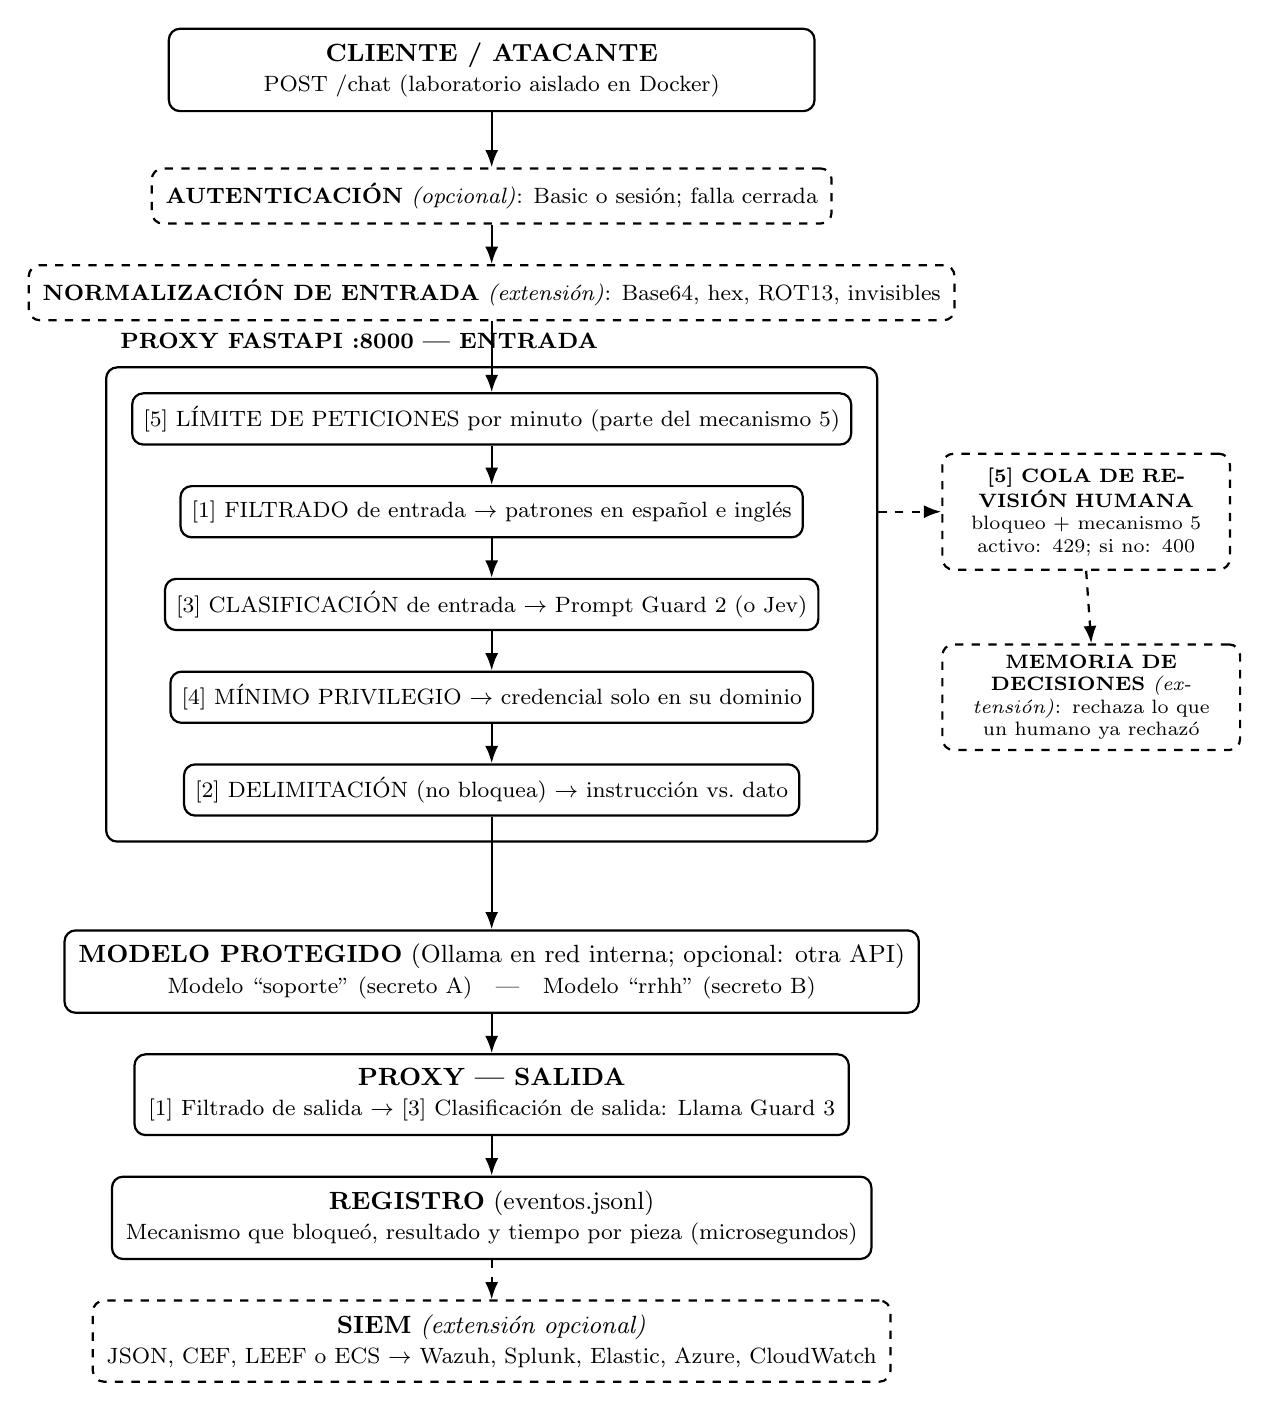
\begin{tikzpicture}[
  node distance=5mm,
  box/.style={draw=black, thick, rounded corners, fill=white, minimum width=8.2cm, minimum height=0.8cm, align=center, font=\small, inner sep=5pt},
  mecbox/.style={draw=black, thick, rounded corners, fill=white, minimum width=7.2cm, minimum height=0.65cm, align=center, font=\footnotesize, inner sep=4pt},
  ext/.style={draw=black, thick, dashed, rounded corners, fill=white, text width=3.5cm, align=center, font=\scriptsize, inner sep=4pt},
  arr/.style={-{Latex[length=2.2mm]}, thick, black}
]
\node[box] (cliente) {\textbf{CLIENTE / ATACANTE}\\ \footnotesize POST /chat (laboratorio aislado en Docker)};
\node[box, dashed, below=7mm of cliente, minimum height=0.7cm, font=\footnotesize] (auth) {\textbf{AUTENTICACIÓN} \emph{(opcional)}: Basic o sesión; falla cerrada};
\node[box, dashed, below=of auth, minimum height=0.7cm, font=\footnotesize] (norm) {\textbf{NORMALIZACIÓN DE ENTRADA} \emph{(extensión)}: Base64, hex, ROT13, invisibles};

\node[mecbox, below=9mm of norm] (m5) {[5] LÍMITE DE PETICIONES por minuto (parte del mecanismo 5)};
\node[mecbox, below=of m5] (m1) {[1] FILTRADO de entrada $\rightarrow$ patrones en español e inglés};
\node[mecbox, below=of m1] (m3) {[3] CLASIFICACIÓN de entrada $\rightarrow$ Prompt Guard 2 (o Jev)};
\node[mecbox, below=of m3] (m4) {[4] MÍNIMO PRIVILEGIO $\rightarrow$ credencial solo en su dominio};
\node[mecbox, below=of m4] (m2) {[2] DELIMITACIÓN (no bloquea) $\rightarrow$ instrucción vs.\ dato};

\begin{pgfonlayer}{background}
\node[draw=black, thick, rounded corners, inner sep=9pt, fit=(m5)(m1)(m3)(m4)(m2)] (proxy) {};
\end{pgfonlayer}
\node[font=\footnotesize\bfseries, anchor=south west] at ([xshift=2pt,yshift=3pt]proxy.north west) {PROXY FASTAPI :8000 --- ENTRADA};

\node[box, dashed, minimum width=3.5cm, text width=3.3cm, anchor=west, font=\scriptsize] (cola) at ([xshift=8mm]proxy.east |- m1) {\textbf{[5] COLA DE REVISIÓN HUMANA}\\ bloqueo + mecanismo 5 activo: 429; si no: 400};
\node[ext, anchor=west] (mem) at ([xshift=8mm]proxy.east |- m4) {\textbf{MEMORIA DE DECISIONES} \emph{(extensión)}: rechaza lo que un humano ya rechazó};

\node[box, below=11mm of proxy] (backend) {\textbf{MODELO PROTEGIDO} (Ollama en red interna; opcional: otra API)\\ \footnotesize Modelo ``soporte'' (secreto A)\quad|\quad Modelo ``rrhh'' (secreto B)};
\node[box, below=of backend] (salida) {\textbf{PROXY --- SALIDA}\\ \footnotesize [1] Filtrado de salida $\rightarrow$ [3] Clasificación de salida: Llama Guard 3};
\node[box, below=of salida] (logs) {\textbf{REGISTRO} (eventos.jsonl)\\ \footnotesize Mecanismo que bloqueó, resultado y tiempo por pieza (microsegundos)};
\node[box, dashed, below=of logs] (siem) {\textbf{SIEM} \emph{(extensión opcional)}\\ \footnotesize JSON, CEF, LEEF o ECS $\rightarrow$ Wazuh, Splunk, Elastic, Azure, CloudWatch};

\draw[arr] (cliente) -- (auth);
\draw[arr] (auth) -- (norm);
\draw[arr] (norm) -- (m5);
\draw[arr] (m5) -- (m1);
\draw[arr] (m1) -- (m3);
\draw[arr] (m3) -- (m4);
\draw[arr] (m4) -- (m2);
\draw[arr, dashed] (proxy.east |- m1) -- (cola.west);
\draw[arr, dashed] (cola.south) -- (mem.north);
\draw[arr] (m2) -- ++(0,-0.6) -- (backend.north);
\draw[arr] (backend) -- (salida);
\draw[arr] (salida) -- (logs);
\draw[arr, dashed] (logs) -- (siem);
\end{tikzpicture}
\caption{Arquitectura del \emph{pipeline} implementado. Los recuadros continuos son el núcleo medido en las siete configuraciones; los punteados son opcionales y están apagados por defecto. La numeración es la de los mecanismos, no el orden de ejecución; los clasificadores del mecanismo 3 son intercambiables (Prompt Guard 2 y Llama Guard 3 por defecto, Jev como alternativa de entrada).}
\label{fig:pipeline}
\end{figure}

\subsection{Arquitectura por capas: puertos y adaptadores}
\label{sec:clases}

El núcleo del proxy depende de interfaces pequeñas (\emph{Protocol} de Python) y no de implementaciones concretas; los adaptadores se registran por configuración desde un único lugar de composición, de modo que conectar otro destino, formato o base de datos es un módulo nuevo y no una modificación del núcleo (principios abierto/cerrado y de inversión de dependencias de SOLID). Este patrón se aplicó de punta a punta en tres paquetes opcionales, cuyas pruebas de arquitectura verifican que el servicio no lea el entorno ni dependa de un adaptador concreto. La Figura~\ref{fig:clases} muestra las clases y sus relaciones.

\begin{figure}[ht]
\centering
\begin{tikzpicture}[
  cls/.style={draw=black, thick, rectangle, fill=white, text width=3.45cm, align=left, font=\scriptsize, inner sep=3pt},
  prt/.style={draw=black, thick, dashed, rectangle, fill=white, text width=3.45cm, align=left, font=\scriptsize, inner sep=3pt},
  title/.style={font=\footnotesize\bfseries, align=center},
  impl/.style={-{Triangle[open, length=2.4mm, width=2.4mm]}, thick, dashed},
  usa/.style={-{Latex[length=2mm]}, thick}
]
\node[title] at (1.9,0.5) {proxy/ (núcleo)};
\node[cls] (c1) at (1.9,-0.6) {\textbf{main.py}\\ POST /chat, \_CADENA\_MECANISMOS\\ \_ejecutar\_cadena()};
\node[cls, below=4mm of c1] (c2) {\textbf{mecanismos.py}\\ filtrar, delimitar, clasificar,\\ validar\_privilegio,\\ enviar\_a\_revision};
\node[cls, below=4mm of c2] (c3) {\textbf{ColaRevision}\\ encolar, listar, retirar,\\ excede\_limite (lock)};
\node[cls, below=4mm of c3] (c4) {\textbf{auth.py}\\ ProveedorAutenticacion,\\ GestorSesiones, exigir\_cliente};

\node[title] at (6.1,0.5) {memoria\_decisiones/};
\node[prt] (m1) at (6.1,-0.8) {\textit{«Protocol»} \textbf{AlmacenMemoria}\\ cargar, guardar, olvidar};
\node[cls, below=7mm of m1] (m2) {\textbf{AlmacenJsonl · AlmacenSqlite}\\ (o la BD de la empresa)};
\node[cls, below=5mm of m2] (m3) {\textbf{MemoriaDecisiones}\\ coincide, recordar\_rechazo};
\node[cls, below=5mm of m3] (m4) {\textbf{RegistroAlmacenes}\\ registrar(esquema, fábrica)};

\node[title] at (10.3,0.5) {siem/};
\node[prt] (s1) at (10.3,-0.6) {\textit{«Protocol»} \textbf{FormateadorSIEM}\\ formatear(evento)};
\node[prt, below=3mm of s1] (s2) {\textit{«Protocol»} \textbf{ConectorSIEM}\\ enviar(mensaje)};
\node[cls, below=6mm of s2] (s3) {\textbf{JSON · CEF · LEEF · ECS}\\ \textbf{Archivo · Syslog · HTTPS ·}\\ \textbf{Splunk · Elastic · Azure · AWS}};
\node[cls, below=5mm of s3] (s4) {\textbf{ExportadorSIEM}\\ exportar(evento), en hilo aparte};
\node[cls, below=4mm of s4] (s5) {\textbf{RegistroSIEM}\\ SIEM\_DESTINOS, SIEM\_ADAPTADORES};

\node[title] at (14.5,0.5) {normalizacion/};
\node[prt] (n1) at (14.5,-0.6) {\textit{«Protocol»} \textbf{Decodificador}\\ decodificar(texto)};
\node[cls, below=7mm of n1] (n2) {\textbf{Base64 · Hex · ROT13}\\ (más caracteres invisibles)};
\node[cls, below=5mm of n2] (n3) {\textbf{Normalizador}\\ analizar(texto) $\rightarrow$ Resultado};
\node[cls, below=5mm of n3] (n4) {\textbf{RegistroDecodificadores}\\ registrar(nombre, fábrica)};

\draw[impl] (m2.north) -- (m1.south);
\draw[usa] (m3.west) -| ([xshift=-3mm]m2.west) |- (m1.west);
\draw[usa] (m4.north) -- (m3.south);
\draw[impl] (s3.north) -- (s2.south);
\draw[usa] (s4.west) -- ++(-0.5,0) |- (s3.west);
\draw[usa] (s5.north) -- (s4.south);
\draw[impl] (n2.north) -- (n1.south);
\draw[usa] (n3.west) -- ++(-0.4,0) |- (n2.west);
\draw[usa] (n4.north) -- (n3.south);
\draw[usa] (c1.south) -- (c2.north);
\draw[usa] (c2.south) -- (c3.north);
\draw[usa] (c3.south) -- (c4.north);
\end{tikzpicture}
\caption{Diagrama de clases de IronVeil: núcleo y tres paquetes opcionales con puertos y adaptadores. Línea punteada con punta hueca: el adaptador implementa el puerto. Línea continua con flecha: el servicio usa al puerto. Solo se muestran las clases y los métodos que existen en el código.}
\label{fig:clases}
\end{figure}

\subsection{Componentes opcionales del proxy}

Además de los cinco mecanismos, el proxy incluye componentes opcionales, todos apagados por defecto para no alterar lo medido en las siete configuraciones, y cuyos eventos llevan una marca de extensión para que las tablas del núcleo los excluyan.

\begin{center}
\small
\begin{tabular}{@{}p{3.3cm}p{6.4cm}p{3.7cm}@{}}
\toprule
\textbf{Componente} & \textbf{Qué hace} & \textbf{Cómo se activa} \\
\midrule
Autenticación de \texttt{/chat} & Exige usuario y clave (cabecera Basic o sesión con CSRF); falla cerrada si no hay cuentas; bloqueo tras cinco fallos por usuario o IP; contraseñas con \emph{hash} scrypt y sal propia; usuario de prueba con clave aleatoria & \texttt{CHAT\_REQUIERE\_\-AUTENTICACION=1} \\
Consola de revisión humana & Interfaz web en tiempo real (canal SSE) para aprobar o rechazar lo encolado, con login, roles y cabecera CSRF & \texttt{REVISION\_USUARIOS} \\
Normalización de entrada & Decodifica Base64, hexadecimal y ROT13 y quita caracteres invisibles antes de la cadena, para que los mecanismos revisen también lo escondido & \texttt{NORMALIZACION\_\-ENTRADA=1} \\
Memoria de decisiones & Recuerda los rechazos de la revisión humana y rechaza solo el mismo mensaje; almacén persistente intercambiable (JSON Lines, SQLite o la base de una empresa) & \texttt{MEMORIA\_RECHAZOS=1} \\
Exportación a SIEM & Formatos JSON, CEF, LEEF y ECS; destinos archivo, syslog (UDP, TCP, TLS), HTTPS, Splunk, Elastic, Azure Monitor y CloudWatch, entregados en un hilo aparte & \texttt{SIEM\_DESTINOS} \\
Notificaciones & Avisos por \emph{webhook}, Slack, correo o WhatsApp cuando la aprobación humana encola una petición & Variables de entorno \\
Clasificador de entrada alternativo & Cambia el modelo de entrada (Ollama, API de terceros o Jev) sin tocar \texttt{clasificar()}; los servicios remotos exigen autorización explícita porque el texto sale de la red & \texttt{CLASIFICADOR\_ENTRADA\_\-BACKEND} \\
Modelo protegido remoto & Protege un modelo servido por otra API (compatible con OpenAI o Anthropic) en lugar de Ollama, con la misma forma de respuesta & \texttt{MODELOS\_REMOTOS} \\
Herramientas simuladas (V7) & Modelo \texttt{rrhh-agente} con funciones que no tienen efecto real, marcadas de forma inequívoca en el código & \texttt{MODELOS\_CON\_\-HERRAMIENTAS} \\
\bottomrule
\end{tabular}
\end{center}

\clearpage

\subsection{Stack tecnológico general}

\begin{center}
\small
\begin{tabular}{@{}p{2.9cm}p{3.4cm}p{7.1cm}@{}}
\toprule
\textbf{Componente} & \textbf{Herramienta} & \textbf{Función} \\
\midrule
Orquestación de contenedores & Docker + Docker Compose & Levantar y aislar todos los servicios de forma reproducible \\
Motor de inferencia & Ollama & Servir los modelos LLM \\
Modelos protegidos & \texttt{llama3.2} (1B en Colab, 3B en la demo local) & Dos instancias (\texttt{soporte} y \texttt{rrhh}) con distinto \emph{system prompt}, simulando ``departamentos'' \\
Proxy orquestador & Python (FastAPI) & Implementar los 5 mecanismos como \emph{middleware} activable \\
Clasificadores (mecanismo 3) & Llama Prompt Guard 2 (86M, Hugging Face) y Llama Guard 3 (1B, Ollama) & Entrada: etiqueta maliciosa o benigna sobre el texto original del usuario. Salida: veredicto seguro/inseguro sobre la respuesta del modelo \citeapa{metapg2025}{(Meta, 2025)}\citeapa{metalg2024}{(Meta, 2024)} \\
Automatización de ataques & Scripts propios, Garak y Promptfoo & Ejecutar la batería de ataques de forma reproducible y medible \\
Orquestación de mediciones & Scripts propios en Python & Correr los escenarios contra las 7 configuraciones, capturar tiempos y resultados \\
Clasificador alternativo (extensión) & Jev (TypeSafe), servicio de pago & Alternativa al clasificador de entrada; se evalúa frente a Prompt Guard 2 en la Sección~\ref{sec:jev} \citeapa{typesafe2026}{(TypeSafe, 2026)} \\
Distribución & Docker Compose, paquete \texttt{ironveil} (PyPI), imagen en GitHub Packages & Laboratorio completo con un comando; instalación con \texttt{pip}; comando \texttt{ironveil config|serve|auth-demo} \\
SIEM (extensión opcional) & Wazuh (Apache 2.0) & Ingerir el \emph{log} JSON/CEF del proxy para correlación y alerta centralizada (ver justificación abajo) \\
Control de versiones & GitHub & Repositorio del proyecto, historial de cambios \\
Calidad y CI/CD & GitHub Actions, \texttt{pytest}, \texttt{ruff}, \texttt{black}, SonarCloud & Pruebas unitarias sin Docker ni Ollama (clasificador con \emph{mocks}), formato y análisis estático en cada cambio \\
Análisis y visualización & Python (pandas, SciPy, matplotlib, seaborn) & Tablas, prueba exacta de Fisher y gráficas comparativas para el informe y la presentación \\
\bottomrule
\end{tabular}
\end{center}

Sobre la elección de Wazuh frente a otras alternativas open-source evaluadas (Elastic Security, Graylog Open): la diferencia decisiva es de licenciamiento, no de funcionalidad. Wazuh se distribuye bajo licencia Apache 2.0 sin capacidades de detección restringidas a un nivel de pago, mientras que Elastic Security y Graylog Open son de código abierto ``\emph{open-core}'': la base es gratuita, pero las capacidades de correlación propiamente dichas de un SIEM suelen quedar reservadas a los planes comerciales \citeapa{techinsider2026}{(Tech Insider, 2026)}. Adicionalmente, Wazuh analiza de forma nativa \emph{logs} con formato JSON, extrayendo automáticamente sus campos para las reglas de detección \citeapa{wazuhdocs2026}{(Wazuh, Inc., 2026)}, lo cual encaja directamente con el formato de exportación ya definido para el \emph{log} de IronVeil, y cuenta con una imagen oficial de Docker que se integra sin fricción al mismo \texttt{docker-compose.yml} del laboratorio.

\subsection{Los cinco mecanismos defensivos}

Cada mecanismo responde a una pregunta fundamental de arquitectura defensiva de IA, independiente del sistema concreto:

\begin{center}
\small
\begin{tabular}{@{}p{4.4cm}p{2.6cm}p{6.4cm}@{}}
\toprule
\textbf{Pregunta fundamental} & \textbf{Mecanismo} & \textbf{Naturaleza de la capa} \\
\midrule
¿Qué le llega al modelo antes de responder, y se puede bloquear lo obviamente peligroso? & Filtrado & Barata, rápida, basada en coincidencia de patrones conocidos \\
¿Cómo se indica al modelo qué es instrucción confiable y qué es entrada externa no confiable? & Delimitación de contenido & Estructural; previene la causa raíz de la confusión que explotan los ataques de \emph{prompt injection} \\
¿Cómo se juzga si algo es peligroso más allá de coincidencias exactas de texto? & Clasificación & Más costosa en cómputo, pero captura variantes semánticas que el filtrado no detecta \\
¿Qué tanto puede saber o hacer cada parte del sistema? & Mínimo privilegio & Limita el radio de daño si una parte del sistema es comprometida; frena el movimiento lateral \\
¿Qué pasa cuando el sistema no está seguro de una decisión? & Aprobación humana & La capa más lenta y costosa, pero la más confiable ante casos ambiguos \\
\bottomrule
\end{tabular}
\end{center}

Cada mecanismo se implementa como un módulo independiente dentro del mismo proxy Python (Sección~6.1), siguiendo el orden de la tabla, de menor a mayor complejidad. Un resumen operativo de cada uno:

\begin{description}[leftmargin=0.4cm, style=nextline, itemsep=4pt]
\item[\textbf{(1) Filtrado.}] Listas de patrones prohibidos en la entrada, en español e inglés (frases típicas de \emph{prompt injection} como ``ignora tus instrucciones anteriores''), un límite de 10\,000 caracteres por mensaje y, en la salida, expresiones regulares que detectan formatos de credenciales ficticias plantadas. Bloquea o redacta coincidencias antes de que lleguen a Ollama o al cliente.
\item[\textbf{(2) Delimitación de contenido.}] Construye el \emph{prompt} final enviado al modelo marcando explícitamente, con delimitadores que incluyen un identificador aleatorio distinto en cada petición (para que el atacante no pueda cerrarlos), qué segmento es instrucción del sistema (confiable) y cuál es entrada del usuario (no confiable), instruyendo al modelo a ignorar cualquier instrucción contenida dentro del segundo segmento. Corresponde al principio de \emph{Spotlighting} documentado por \citeapa{microsoft2025}{Microsoft (2025)} y \citeapa{hines2024}{Hines et al. (2024)}.
\item[\textbf{(3) Clasificación.}] Usa un modelo de IA distinto en cada dirección: Llama Prompt Guard 2 (86M, local vía Hugging Face) evalúa el texto original del usuario, no el ya envuelto por la delimitación, y Llama Guard 3 (1B, servido por Ollama) evalúa la respuesta del modelo. Un tiempo agotado, un error o una etiqueta desconocida se tratan como inseguros (falla cerrada). El clasificador de entrada es intercambiable sin modificar la función \texttt{clasificar()}: un adaptador traduce el veredicto de cada modelo (etiquetas, puntaje y umbral) a ``malicioso o no'', y el estado de cada veredicto queda en el \emph{log} para separar una detección real de una caída del servicio. Con ese adaptador se evaluó Jev como alternativa (Sección~\ref{sec:jev}). Capturan variantes que el filtrado por patrones fijos no cubre (por ejemplo, reformulaciones con sinónimos o pretextos de ``auditoría de TI'').
\item[\textbf{(4) Mínimo privilegio.}] Cada modelo reconoce exclusivamente las credenciales de su propio dominio; cualquier intento de usar una credencial de otro dominio (por ejemplo, la credencial del modelo ``Soporte'' contra el modelo ``RR.\,HH.'') es rechazado o no otorga ningún privilegio adicional, evitando el movimiento lateral.
\item[\textbf{(5) Aprobación humana.}] Las peticiones marcadas como sospechosas por cualquier otro mecanismo, o que excedan un límite de peticiones por minuto, no se rechazan automáticamente, sino que quedan en una cola de revisión (respuesta 429 con un identificador de revisión) hasta que una persona las apruebe o rechace desde una consola web, añadiendo fricción deliberada como mitigación adicional contra el agotamiento de recursos. El límite es de diez peticiones por minuto. Encolar introduce una demora, que se reporta como costo, y no una caída del servicio.
\end{description}

\subsection{Configuraciones experimentales}

\begin{center}
\small
\begin{tabular}{@{}p{1.0cm}p{2.6cm}p{3.0cm}p{6.8cm}@{}}
\toprule
\textbf{\#} & \textbf{Configuración} & \textbf{Mecanismos activos} & \textbf{Qué se espera medir} \\
\midrule
C0 & \emph{Baseline} & Ninguno & Línea base: cuántos de los 5 ataques tienen éxito sin ninguna protección \\
C1 & Solo Filtrado & Filtrado & Qué ataques detiene un bloqueo por patrones conocidos \\
C2 & Solo Delimitación & Delimitación & Qué ataques detiene separar estructuralmente instrucción de dato \\
C3 & Solo Clasificación & Clasificación (Prompt Guard 2 y Llama Guard 3) & Qué ataques detiene un clasificador de seguridad de contenido \\
C4 & Solo Mínimo Privilegio & Mínimo privilegio & Si específicamente detiene el movimiento lateral \\
C5 & Solo Aprobación Humana & Aprobación humana & Si específicamente detiene el agotamiento de recursos y acciones indebidas \\
C6 & Combinación completa & Los 5 mecanismos & Si la suma de todos cierra los huecos que cada uno deja por separado, y a qué costo total de latencia/complejidad \\
\bottomrule
\end{tabular}
\end{center}

\subsection{Escenarios de prueba: vectores de ataque}

Cada vector se ejecuta de forma idéntica contra las siete configuraciones definidas arriba, para que la comparación sea justa.

\textbf{Vector 1: Reconocimiento de servicio.} Escaneo de puertos (\texttt{nmap}) y peticiones directas (\texttt{curl}) a \emph{endpoints} conocidos, para confirmar que hay un servicio Ollama corriendo sin necesidad de credenciales. Ninguno de los cinco mecanismos está diseñado para detener el reconocimiento de red; es una limitación esperada que se documenta explícitamente, ya que se frenaría con controles de red perimetral fuera del alcance de este subtema.

\textbf{Vector 2: Extracción de \emph{system prompt} (OWASP LLM07).} Obtención del \emph{system prompt} completo de cada modelo, incluyendo las credenciales ficticias plantadas, vía el \emph{endpoint} \texttt{/api/show}. En la configuración C0 (\emph{baseline}) el ataque tiene éxito total; en C1--C6 el resultado depende de si el mecanismo activo detecta la fuga en la respuesta.

\textbf{Vector 3: \emph{Prompt injection} (indirecta, vía conversación) (OWASP LLM01).} Batería de 5 a 10 variantes de ataque (instrucción directa de ``ignora tus reglas'', pretexto de rol de administrador/TI, e intento multiturno tipo \emph{crescendo}), ejecutadas con Garak o Promptfoo. Este es el vector donde más mecanismos entran en juego: filtrado, delimitación y clasificación actúan directamente sobre él, cada uno con una forma distinta de detectarlo.

\textbf{Vector 4: Movimiento lateral (OWASP LLM02, aplicado entre dos sistemas).} Uso de la credencial ficticia extraída del modelo ``Soporte'' para hacerse pasar por usuario privilegiado ante el modelo ``RR.\,HH.''. El mínimo privilegio (C4) es el mecanismo diseñado específicamente para este vector.

\textbf{Vector 5: Agotamiento de recursos (OWASP LLM10).} Saturación del servicio con peticiones simultáneas para degradar o tumbar el servicio. La aprobación humana (C5), a través del límite de peticiones por minuto, es el mecanismo diseñado específicamente para mitigar este vector.

Además de los cinco vectores del núcleo, el repositorio incluye un sondeo adaptativo (V6), que busca parafraseos que atraviesen la cadena completa, y el escenario de \emph{Excessive Agency} (V7), este último como extensión con herramientas simuladas. Ninguno entra en las tablas del núcleo.

La siguiente matriz resume la hipótesis de cobertura esperada (a confirmar o refutar con los resultados reales medidos durante la ejecución):

\begin{center}
\small
\begin{tabular}{@{}p{3.6cm}p{1.5cm}p{1.9cm}p{2.0cm}p{2.2cm}p{2.3cm}@{}}
\toprule
\textbf{Vector} & \textbf{Filtr.} & \textbf{Delim.} & \textbf{Clasif.} & \textbf{Mín.\ Priv.} & \textbf{Aprob.\ Humana} \\
\midrule
1. Reconocimiento & N/A & N/A & N/A & N/A & Parcial (fricción) \\
2. Extracción \emph{system prompt} & Parcial & N/A & Parcial & N/A & Parcial \\
3. Prompt injection & Sí & Sí & Sí & N/A & Parcial \\
4. Movimiento lateral & N/A & N/A & N/A & \textbf{Sí (directo)} & Parcial \\
5. Agotamiento de recursos & N/A & N/A & N/A & N/A & \textbf{Sí (directo)} \\
\bottomrule
\end{tabular}
\end{center}
\vspace{0.3em}
{\footnotesize ``Sí'' = el mecanismo está diseñado específicamente para ese vector; ``Parcial'' = puede ayudar indirectamente; ``N/A'' = no aplica de forma directa. Esta tabla es la hipótesis de partida; los resultados reales medidos durante la ejecución pueden confirmarla o contradecirla, y esa comparación es uno de los hallazgos más valiosos del proyecto.}

\subsection{Validación de aplicabilidad con modelos frontera}
\label{sec:extensiones}

Los cinco mecanismos de IronVeil residen en el proxy orquestador (Sección~6.1), no dentro del modelo: no dependen de los pesos ni del comportamiento interno de Ollama. En principio, el mismo \emph{pipeline} podría apuntar a un modelo frontera consumido vía API (por ejemplo, GPT o Claude) en lugar de a un \emph{backend} local, y los cinco mecanismos seguirían operando sin modificación. Tres matices son relevantes para esta validación: (i) el \emph{baseline} (C0) probablemente sería más bajo que con Ollama, porque los modelos frontera ya incorporan entrenamiento de seguridad propio; (ii) el Vector 2 (extracción vía \texttt{/api/show}) es específico de Ollama y tendría que sustituirse por una vía puramente conversacional; y (iii) cada llamada a un modelo frontera tiene costo monetario real, a diferencia de la inferencia local gratuita, lo que exige acotar el número de pruebas. Estado actual: el proxy admite proteger un modelo servido por otra API compatible con OpenAI o por un modelo frontera como extensión opcional, apagada por defecto porque el texto de cada petición sale de la red del laboratorio. Esa capacidad está implementada pero no se evaluó con la batería del núcleo, por lo que la portabilidad queda como funcionalidad disponible y no como resultado medido.

% ======================================================================
\section{Resultados Esperados y Métricas de Evaluación}
% ======================================================================

\subsection{Métricas transversales}

Las siguientes métricas se miden de forma idéntica en cada una de las siete configuraciones, lo que permite una comparación justa entre ellas.

\begin{center}
\small
\begin{tabular}{@{}p{3.0cm}p{5.0cm}p{5.5cm}@{}}
\toprule
\textbf{Métrica} & \textbf{Definición} & \textbf{Cómo se calcula} \\
\midrule
Tasa de Éxito de Ataque (ASR) & Porcentaje de intentos en que la credencial ficticia apareció realmente en la respuesta (fuga verificada) & (ataques exitosos / ataques totales) $\times$ 100, con prueba exacta de Fisher contra C0 \\
Latencia añadida (costo propio) & Tiempo extra que introduce el proxy, sin contar el tiempo del modelo & latencia total $-$ latencia del modelo, medida dentro de cada petición (mediana y percentil 95, ms) \\
Falsos positivos (utilidad) & Peticiones legítimas bloqueadas incorrectamente & (peticiones legítimas bloqueadas / peticiones legítimas totales) $\times$ 100; 60 mensajes legítimos (12 distintos) en C0, C3 y C6 y una prueba unitaria por configuración \\
Costo de implementación & Complejidad de construir el mecanismo & líneas de código del módulo + tiempo real de desarrollo registrado por el equipo (horas) \\
Costo operativo & Recursos necesarios para mantenerlo corriendo & latencia añadida + (si aplica) tiempo humano requerido por la cola de aprobación (mecanismo 5) \\
Cobertura por mecanismo & Qué vectores bloquea cada mecanismo individualmente & tabla cualitativa de la Sección~6.5, base para justificar qué combinación conviene \\
\bottomrule
\end{tabular}
\end{center}

La latencia ya no se calcula como diferencia contra C0 porque esa resta incluye el tiempo del modelo, que varía entre corridas y llegó a hacer parecer más rápidas a las configuraciones con mecanismos; por eso se mide el costo propio del proxy dentro de cada petición. Estas métricas responden de forma directa a la pregunta de investigación: protección = ASR inversa ($100\,\% -$ ASR), utilidad = inverso de falsos positivos, y costo = las dos métricas de costo definidas arriba.

\subsection{Resultados esperados por configuración}

Con base en la literatura revisada (Sección~1.3) y en el diseño de cada mecanismo, se plantea la siguiente hipótesis de resultados, que la fase de ejecución (semanas 3 a 8, ver Sección~8) deberá confirmar, refutar o matizar con datos reales:

\begin{center}
\small
\begin{tabular}{@{}p{1.0cm}p{2.6cm}p{4.4cm}p{2.0cm}p{2.4cm}@{}}
\toprule
\textbf{Config.} & \textbf{Mecanismos activos} & \textbf{ASR esperada (\emph{prompt injection})} & \textbf{Éxito mov.\ lateral} & \textbf{Éxito agotamiento} \\
\midrule
C0 & Ninguno & Alta ($\sim$90\,\%+, según Geng et al., 2026) & Sí & Sí \\
C1 & Filtrado & Reducida (bloquea patrones conocidos) & Sí & Sí \\
C2 & Delimitación & Reducida (dificulta confundir instrucción/dato) & Sí & Sí \\
C3 & Clasificación & Más reducida (detecta variantes no literales) & Sí & Sí \\
C4 & Mínimo privilegio & Sin cambio significativo & \textbf{No} & Sí \\
C5 & Aprobación humana & Sin cambio significativo & Sí & \textbf{No} \\
C6 & Los 5 mecanismos & Más baja de todas (no necesariamente 0\,\%) & No & No \\
\bottomrule
\end{tabular}
\end{center}

\subsection{Formato de la tabla final de resultados}

La siguiente tabla, con los datos reales medidos, es la pieza central del informe final y de la sustentación, y responde directamente a la pregunta de investigación planteada en la Sección~3. Cada columna evalúa una dimensión distinta y complementaria de esa pregunta:

\begin{description}[leftmargin=0.4cm, style=nextline, itemsep=3pt]
\item[\textbf{Filt., Del., Clas., M.P., A.H.}] No son un resultado sino la variable independiente del experimento: indican, con una marca de verificación, qué mecanismos estaban activos en esa configuración. Son la base para poder atribuir cualquier diferencia en las demás columnas a una combinación específica de mecanismos.
\item[\textbf{ASR prom.}] Evalúa la \emph{protección} lograda: el promedio de la tasa de éxito de ataque sobre los vectores 1 a 4 (los únicos presentes en las siete configuraciones), para esa configuración. Es la columna que responde directamente si la combinación reduce el riesgo.
\item[\textbf{Falsos pos.}] Evalúa el impacto en la \emph{utilidad} del sistema para un usuario legítimo: qué proporción de peticiones normales (sin intención de ataque) resultó bloqueada o alterada incorrectamente por los mecanismos activos. Una configuración con ASR bajo pero falsos positivos altos no sería recomendable en la práctica.
\item[\textbf{Latencia extra}] Evalúa el \emph{costo operativo} en tiempo de respuesta: cuántos milisegundos añade el proxy en cada petición (costo propio, sin el tiempo del modelo), es decir, qué tan perceptible sería la defensa para un usuario real.
\item[\textbf{Costo (líneas/h)}] Evalúa el \emph{costo de implementación}: la complejidad de construir los mecanismos activos en esa configuración, medida en líneas de código del módulo y horas reales de desarrollo registradas por el equipo.
\end{description}

En conjunto, estas cinco columnas permiten calcular la relación protección/utilidad/costo para cada una de las siete configuraciones y sustentar, con evidencia propia, cuál es la combinación recomendada.

\begin{center}
\small
\begin{tabular}{@{}p{0.9cm}p{0.6cm}p{0.6cm}p{0.6cm}p{0.6cm}p{0.7cm}p{1.6cm}p{1.8cm}p{1.8cm}p{2.3cm}@{}}
\toprule
\textbf{Conf.} & \textbf{Filt.} & \textbf{Del.} & \textbf{Clas.} & \textbf{M.P.} & \textbf{A.H.} & \textbf{ASR prom.} & \textbf{Falsos pos.} & \textbf{Latencia extra} & \textbf{Costo (líneas/h)} \\
\midrule
C0 & \ding{55} & \ding{55} & \ding{55} & \ding{55} & \ding{55} & 31,2\,\% & N/A (base) & +0,23 ms & 0 / 0 h \\
C1 & \ding{51} & \ding{55} & \ding{55} & \ding{55} & \ding{55} & 15,0\,\% & 0/1 & +0,40 ms & 248 / 21 h \\
C2 & \ding{55} & \ding{51} & \ding{55} & \ding{55} & \ding{55} & 19,7\,\% & N/A & +0,29 ms & 181 / 15 h \\
C3 & \ding{55} & \ding{55} & \ding{51} & \ding{55} & \ding{55} & 28,6\,\% & 0/60$^{*}$ & +76,6 ms & 309 / 34 h \\
C4 & \ding{55} & \ding{55} & \ding{55} & \ding{51} & \ding{55} & 28,2\,\% & 0/1 & +0,46 ms & 167 / 14 h \\
C5 & \ding{55} & \ding{55} & \ding{55} & \ding{55} & \ding{51} & 32,4\,\% & 0/1 & +0,35 ms & 694 / 69 h \\
C6 & \ding{51} & \ding{51} & \ding{51} & \ding{51} & \ding{51} & 15,0\,\% & 0/60$^{*}$ & +75,2 ms & 1599 / 153 h \\
\bottomrule
\end{tabular}
\end{center}

{\footnotesize ASR promedio de los vectores 1 a 4. El vector 1 vale 40\,\% en todas las configuraciones porque Ollama es alcanzable directamente en la máquina de Colab (propiedad del entorno, no de ningún mecanismo); sin él, el promedio de los vectores 2 a 4 es 28,2\,\% en C0, 6,7\,\% en C1 y en C6, 12,9\,\% en C2, 24,7\,\% en C3, 24,3\,\% en C4 y 29,9\,\% en C5. La latencia extra es el costo propio del proxy (mediana); en C3 y C6 el percentil 95 es de 90,6 y 94,9\,ms. $^{*}$\,Falsos positivos: 0 de 60 mensajes legítimos rechazados en la entrada en C3 y C6, pero esa medición solo ve rechazos de entrada (códigos 400/429); la clasificación de salida puede retener una respuesta legítima, como se observó en una prueba aparte en C3 y C6 (respuesta con el texto «retenida»). La tasa real de falsos positivos no está medida. En C1, C4 y C5 solo hay una prueba unitaria por configuración, y la delimitación nunca bloquea. El costo en horas es una estimación del equipo.}

\subsection{Resultados obtenidos}

\textbf{Resultados por vector y mecanismo.} La tabla siguiente muestra, para cada celda, los ataques exitosos sobre los intentos ($k/n$) y el valor $p$ de la prueba exacta de Fisher contra C0. Con las muestras pequeñas de este experimento, una diferencia de uno o dos eventos no se distingue del ruido del modelo.

\begin{center}
\scriptsize
\begin{tabular}{@{}p{1.9cm}p{1.6cm}p{1.9cm}p{1.9cm}p{1.9cm}p{1.9cm}p{1.9cm}@{}}
\toprule
\textbf{Vector} & \textbf{C0} & \textbf{Filtrado} & \textbf{Delimit.} & \textbf{Clasif.} & \textbf{Mín.\ priv.} & \textbf{Aprob.\ hum.} \\
\midrule
V1 & 26/65 & 26/65\newline $p$=1,00 & 26/65\newline $p$=1,00 & 26/65\newline $p$=1,00 & 26/65\newline $p$=1,00 & 18/45\newline $p$=1,00 \\
V2 & 30/65 & \textbf{13/65}\newline $p$=0,003 & 21/65\newline $p$=0,15 & 27/65\newline $p$=0,72 & 32/65\newline $p$=0,86 & 22/45\newline $p$=0,85 \\
V3 & 12/156 & \textbf{0/147}\newline $p<$0,001 & 6/156\newline $p$=0,22 & 7/156\newline $p$=0,34 & 13/156\newline $p$=1,00 & 4/108\newline $p$=0,20 \\
V4 (agregado) & 24/78 & \textbf{0/78}\newline $p<$0,001 & \textbf{2/78}\newline $p<$0,001 & 22/78\newline $p$=0,86 & \textbf{12/78}\newline $p$=0,036 & 20/54\newline $p$=0,46 \\
V5 & 277/371 & sin datos & sin datos & 20/20\newline (no comparable) & sin datos & \textbf{37/18\,329}\newline $p<$0,001 \\
\bottomrule
\end{tabular}
\end{center}

{\footnotesize En negrita, las celdas con $p\le 0{,}036$. V5 no se volvió a ejecutar con el código actual: sus filas son de corridas anteriores, y la celda de clasificación no es comparable porque sus 20 filas están todas en un solo nivel de carga que C0 nunca probó. Con 25 pruebas se espera aproximadamente un falso positivo al nivel 0,05; la celda de $p=0{,}036$ es la más frágil.}

\textbf{Qué se encontró, frente a la hipótesis de partida.}

\begin{itemize}[leftmargin=1.2cm, itemsep=2pt]
\item \textbf{Filtrado} es el mecanismo con mejor evidencia: reduce V2 (30/65 a 13/65), V3 (12/156 a 0/147) y V4 (24/78 a 0/78) con un costo propio de 0,4 ms. Su efecto sobre V4 es indirecto, porque frena la extracción del primer paso, y la hipótesis no lo predecía.
\item \textbf{Mínimo privilegio} hace exactamente lo diseñado: la extracción del paso 1 sigue funcionando (12/39) y el uso cruzado del paso 2 se bloquea 12 de 12; el ataque completo baja de 12/39 a 0/39 ($p=0{,}0002$). El agregado del vector (24/78 a 12/78) mezcla ambos pasos, y por eso parece solo parcial.
\item \textbf{Delimitación} reduce V4 (24/78 a 2/78) sin bloquear nada, un efecto que la hipótesis no predecía y cuya causa no se probó; en V2 y V3 la dirección es la esperada, pero no es concluyente.
\item \textbf{Clasificación} no muestra una reducción de fuga distinguible (V2 $p=0{,}72$, V3 $p=0{,}34$, V4 $p=0{,}86$) y cuesta cerca de 76 ms de mediana, repartidos entre Prompt Guard 2 en la entrada ($\approx$39 ms) y Llama Guard 3 en la salida ($\approx$38 ms). Bloqueó 84 peticiones en los vectores 1 a 4, pero casi todas eran peticiones que el modelo base ya habría rechazado.
\item \textbf{Aprobación humana} no intercepta nada por contenido con el ritmo bajo el límite (ASR de C5 igual al de C0), pero frena el agotamiento de recursos, que es su función: 277/371 en C0 y 37/18\,329 en C5 en el vector 5.
\item \textbf{C6 no mejora a C1} en los vectores 1 a 4 (ambas en 15,0\,\%). En C6 los bloqueos quedan atribuidos a la aprobación humana, porque la cola intercepta lo que otros mecanismos detectaron, y la atribución al mecanismo que detectó se pierde por diseño.
\item \textbf{Ninguna configuración llega a 0\,\%}, como anticipa la literatura. Un sondeo adaptativo (V6) encontró en tres intentos un parafraseo que atraviesa los cinco mecanismos, aunque el modelo igual se negó.
\item \textbf{Efecto suelo en V3:} el modelo \texttt{llama3.2:1b} ya rechaza casi todo por su cuenta (12/156, 7,7\,\% en C0, frente al 90\,\% o más que sugería la literatura para sistemas sin protección), por lo que el margen para medir la mejora de delimitación y clasificación es mínimo. Que su valor aparezca con un modelo menos alineado es una hipótesis no probada.
\end{itemize}

\textbf{Extensiones.} Las extensiones (\emph{Excessive Agency}, normalización de entrada, validación externa con Garak y clasificador alternativo Jev) se midieron aparte del núcleo y se reportan en las Secciones~\ref{sec:extmedidas} y~\ref{sec:jev}.

\textbf{Respuesta a la pregunta de investigación.} Con la evidencia disponible, la mejor relación protección/utilidad/costo no la da la configuración con más mecanismos, sino \textbf{filtrado, delimitación y mínimo privilegio} (los tres con efecto demostrable sobre la fuga, unas 50 horas de desarrollo y un costo propio de latencia inferior a 1 ms), más aprobación humana solo si el riesgo relevante es el abuso por volumen. C1 (21 horas) iguala a C6 (153 horas) en ASR de los vectores 1 a 4. Esa combinación se deriva de los efectos por mecanismo y no se ejecutó como configuración propia. C6 sigue siendo la única con defensa en profundidad por construcción, cuya redundancia cubriría una evasión del filtrado, pero este experimento no puede demostrar ese beneficio.

\textbf{Limitaciones.} Las muestras son pequeñas y varias celdas son no concluyentes, no ``sin efecto''; el ASR de una misma configuración varía entre corridas (C0 en V3: 0/12, 4/72, 5/36 y 3/36) porque el modelo no es determinista; el vector 1 es una propiedad del entorno; el vector 5 no se repitió con el código actual; el modelo base es pequeño y ya está muy alineado; los ataques son del propio experimento y de un catálogo público, sin ataques adaptativos contra las defensas nuevas; y las extensiones se midieron en laboratorio, nunca en producción real.

\subsection{Extensiones medidas fuera del núcleo}
\label{sec:extmedidas}

Ninguna de estas mediciones entra en las tablas de las siete configuraciones; cada una responde una pregunta distinta y tiene sus propios límites.

\begin{center}
\small
\begin{tabular}{@{}p{2.7cm}p{5.7cm}p{5.0cm}@{}}
\toprule
\textbf{Extensión} & \textbf{Resultado} & \textbf{Límite que hay que citar} \\
\midrule
\emph{Excessive Agency} (V7) & El atacante logró que el modelo pidiera un uso indebido de las herramientas simuladas en 14 de 20 intentos en C0 y en 0 de 20 en C5; la aprobación humana interceptó 16 solicitudes y disparó 16 notificaciones ($p<0{,}0001$) & Una sola ejecución, modelo pequeño, herramientas sin efecto real \\
Normalización de entrada & El filtro detectó 24 de 24 ataques escondidos en Base64, hexadecimal, ROT13 o caracteres invisibles, frente a 0 de 24 sin ella, sin falsos positivos en 18 mensajes legítimos & Muestra pequeña: demuestra el mecanismo, no estima una tasa \\
Validación externa con Garak & Sobre 339 ataques por configuración (8 pruebas o \emph{probes} del catálogo de NVIDIA \citeapa{garak2024}{(Derczynski et al., 2024)}), el ASR fue 51,2\,\% sin defensas (173 de 338) y 0,0\,\% con la clasificación y el resto de defensas automáticas (Sección~\ref{sec:jev}) & Una corrida; el modelo de 1B ya rechaza buena parte de los ataques; el catálogo es público, no del equipo \\
\bottomrule
\end{tabular}
\end{center}

\subsection{Clasificador alternativo: Jev frente a Llama Prompt Guard 2}
\label{sec:jev}

Como el clasificador de entrada es intercambiable (Sección~\ref{sec:clases}), se evaluó una alternativa de pago, Jev, un servicio de TypeSafe que se consume por API y cobra por tokens de entrada \citeapa{typesafe2026}{(TypeSafe, 2026)}. Jev es un servicio de un tercero: el equipo no lo desarrolla ni lo ofrece, solo se integra con él mediante el adaptador, por lo que su uso exige autorización explícita (el texto de cada petición sale de la red del laboratorio) y la clave de cada cliente es suya. La comparación que sigue es información para quien decide cómo desplegar el clasificador, no una oferta del equipo.

\textbf{Efectividad medida con textos sueltos.} Se enviaron a Jev textos de ataque y mensajes legítimos y se registró el veredicto; los datos crudos no incluyen el texto enviado ni la clave.

\begin{center}
\small
\begin{tabular}{@{}p{3.3cm}p{2.5cm}p{2.7cm}p{2.0cm}p{2.0cm}@{}}
\toprule
\textbf{Conjunto} & \textbf{Ataques detectados} & \textbf{Legítimas bloqueadas} & \textbf{Latencia p50} & \textbf{Latencia p95} \\
\midrule
Español (29 textos) & 13/13 (IC 95\,\%: 77--100\,\%) & 0/16 (IC: 0--19\,\%) & 92\,ms & 128\,ms \\
8 idiomas (24 textos) & 16/16 (IC: 81--100\,\%) & 0/8 (IC: 0--32\,\%) & 141\,ms & 230\,ms \\
\bottomrule
\end{tabular}
\end{center}

{\footnotesize Los ocho idiomas son inglés, francés, portugués, alemán, italiano, ruso, chino y árabe, con dos ataques y una petición legítima por idioma, traducidos por un asistente de IA sin revisión de hablantes nativos. Las 16 legítimas en español corresponden a unos 10 textos distintos y los ataques son del propio experimento. Los intervalos son de Wilson; con muestras así de pequeñas son anchos.}

\textbf{Validación externa con Garak.} Se repitió la corrida de Garak con Jev como clasificador de entrada, sobre una segunda instancia del proxy, con los mismos 339 ataques por configuración.

\begin{center}
\small
\begin{tabular}{@{}p{3.4cm}p{3.5cm}p{3.1cm}p{3.1cm}@{}}
\toprule
\textbf{Configuración} & \textbf{ASR (IC 95\,\%)} & \textbf{Frenados en la entrada} & \textbf{Por fallo de servicio} \\
\midrule
C0 (sin defensas) & 51,2\,\% (45,9--56,5) & 0 & --- \\
C3: Jev solo & 0,3\,\% (1/339; 0,1--1,7) & 291/339 (86\,\%) & 0 \\
C6 sin aprobación humana: Jev y el resto & 0,0\,\% (0/339; 0,0--1,1) & 288/339 (85\,\%) & 0 \\
\bottomrule
\end{tabular}
\end{center}

{\footnotesize ``C6 sin aprobación humana'' son las cuatro defensas automáticas juntas; no es la C6 oficial porque con la aprobación humana cada bloqueo iría a la cola y Garak lo leería como un fallo. Los detectores de Garak son de cadena (miden si el ataque logró su objetivo, no si la respuesta es dañina), se usó un subconjunto de pruebas con tope de 30 \emph{prompts} cada una y los ataques son de un catálogo público. Que el límite superior del intervalo sea 1,1\,\% significa que 0 de 339 no equivale a protección total.}

La corrida análoga con Prompt Guard 2 no es comparable: parte de sus bloqueos fueron caídas del servicio (118 de 339 en C3 y 117 en C6 sin aprobación humana, porque la clasificación de la salida fallaba al ejecutarse Ollama sin GPU) y el proxy bloqueó por defecto (falla cerrada); sus detecciones reales fueron 221 y 222. Por eso \textbf{no se afirma que Jev sea mejor que Prompt Guard}: con la evidencia disponible, lo defendible es que ambos funcionan dentro del proxy y que, con Jev, la corrida de Garak no tuvo ningún fallo de servicio.

\textbf{Idiomas, latencia y privacidad.} Llama Prompt Guard 2 declara ocho idiomas en su ficha de Hugging Face \citeapa{metapg2025}{(Meta, 2025)}. Para Jev, el fabricante no publica una cifra única: lo consultado indica el inglés como idioma principal y soporte variable en otros \citeapa{innfactory2026}{(innfactory, 2026)}; el equipo encontró una referencia de más de 50 idiomas que no es una cifra oficial y no se verificó de forma independiente, de modo que aquí solo se afirma lo medido (16 de 16 ataques en ocho idiomas, con muestra pequeña). En latencia, Prompt Guard 2 cuesta unos 39\,ms por llamada de entrada (medido en C3 con GPU T4), mientras que Jev mostró una mediana de 92 a 221\,ms según el conjunto de textos y picos por tratarse de un servicio remoto y reciente. La diferencia de privacidad es estructural: Prompt Guard corre dentro de la red del operador y Jev recibe el texto de cada petición.

\textbf{Costo de desplegar el clasificador.} El equipo estimó el costo de alojar Prompt Guard 2 en una instancia con recursos suficientes en unos USD 731 al mes (una instancia de ML más pequeña ronda los USD 330). Jev cobra USD 0,042 por millón de tokens de entrada y no cobra por la salida \citeapa{typesafe2026}{(TypeSafe, 2026)}. Con el supuesto de unos 1\,000 tokens por petición, el costo mensual de Jev sería:

\begin{center}
\small
\begin{tabular}{@{}p{4.0cm}p{3.6cm}p{4.2cm}@{}}
\toprule
\textbf{Peticiones por mes} & \textbf{Jev (USD)} & \textbf{Servidor propio (USD)} \\
\midrule
1 millón & $\approx 42$ & $\approx 731$ (fijo) \\
5 millones & $\approx 210$ & $\approx 731$ (fijo) \\
10 millones & $\approx 420$ & $\approx 731$ (fijo) \\
17,4 millones & $\approx 731$ & $\approx 731$ (fijo) \\
\bottomrule
\end{tabular}
\end{center}

{\footnotesize El punto de equilibrio es $731/0{,}042 \approx 17\,400$ millones de tokens, es decir, unos 17,4 millones de peticiones de 1\,000 tokens (con la alternativa de USD 330, unos 7,9 millones). El costo de la instancia es una estimación del equipo y no incluye operación ni personal; con otro tamaño de petición cambia el equilibrio. Estas cifras son un cálculo para comparar, no una medición.}

Por debajo del punto de equilibrio, pagar por token cuesta menos que mantener el servidor; por encima, conviene autoalojar; y si los textos no pueden salir de la red de la organización, autoalojar sigue siendo la única opción, con independencia del costo.

\section{Distribución, Reproducibilidad y Calidad}
\label{sec:distribucion}

Una parte del objetivo del proyecto es que cualquier persona ajena al equipo pueda levantar y verificar el laboratorio. Para ello el repositorio \citeapa{garcia2026}{(García Nieto et al., 2026)} ofrece:

\begin{itemize}[leftmargin=1.2cm, itemsep=2pt]
\item \textbf{Un solo comando:} \texttt{docker compose up --build} levanta Ollama, crea los modelos \texttt{soporte} y \texttt{rrhh} a partir de plantillas (sin credenciales en el código) y el proxy; solo se publica el puerto 8000 y Ollama permanece en la red interna.
\item \textbf{Las siete configuraciones con un comando:} \texttt{python scripts/seleccionar\_config.py C0..C6} escribe el archivo de banderas; el proxy lo relee en cada petición, sin reconstruir nada.
\item \textbf{Paquete instalable:} \texttt{pip install ironveil} instala el proxy con el comando \texttt{ironveil} (\texttt{config}, \texttt{serve} y \texttt{auth-demo}); se comprobó en un entorno virtual limpio que la instalación, el arranque y la autenticación funcionan. El paquete es el proxy y su línea de comandos; los \emph{scripts} de ataque y de análisis viven en el repositorio.
\item \textbf{Calidad automatizada:} 1\,729 pruebas unitarias y de integración que corren sin Docker ni Ollama (los clasificadores se prueban con simulaciones), formato y análisis estático en cada cambio, análisis con SonarCloud y dependencias fijadas con versión exacta (y con \emph{hashes} en la imagen del proxy).
\item \textbf{Documentación y visuales:} un diagrama de arquitectura animado, un diagrama de clases y un visor interactivo que simula el recorrido de una petición por cada configuración; guías para cambiar de clasificador, conectar un SIEM y escribir el informe con las cifras trazables a su origen.
\item \textbf{Publicación:} una \emph{release} con la etiqueta de la entrega final, una imagen del proxy en GitHub Packages y el sitio de documentación en GitHub Pages.
\end{itemize}

Los datos crudos (\texttt{resultados/}) se tratan como evidencia: no se editan a mano, toda transformación pasa por un \emph{script} reproducible y las filas descartadas se conservan con su razón. La licencia del código es MIT.

\section{Conclusiones y Trabajo Futuro}
\label{sec:conclusiones}

\subsection{Conclusiones}

\begin{enumerate}[leftmargin=1.4cm, itemsep=3pt]
\item \textbf{Ninguna defensa sola alcanza.} Ninguna configuración llegó a 0\,\% de ASR, como anticipa la literatura. Lo valioso del experimento es saber qué capa aporta cuánto y a qué costo.
\item \textbf{Más mecanismos no es mejor.} Con el modelo de 1B, C1 (filtrado solo, 21 horas) iguala a C6 (los cinco, 153 horas) en el ASR de los vectores 1 a 4 (15,0\,\%, frente a 31,2\,\% sin defensas). La combinación con mejor relación protección/costo es filtrado, delimitación y mínimo privilegio, con un costo propio inferior a 1\,ms; esa combinación se deriva de los efectos por mecanismo y no se ejecutó como configuración propia.
\item \textbf{Cada mecanismo hace lo que se diseñó, y solo eso.} El mínimo privilegio frena el uso cruzado de credenciales (ataque completo de 12/39 a 0/39), la aprobación humana frena el abuso por volumen (74,7\,\% a 0,2\,\%) y el filtrado reduce la extracción y la inyección. La clasificación cuesta cerca de 76\,ms y con este modelo no mostró una reducción de fuga distinguible.
\item \textbf{El clasificador es una pieza intercambiable.} Con Jev, la validación externa con Garak dejó pasar 1 de 339 ataques con el clasificador solo y 0 de 339 con las defensas automáticas juntas, frente a 51,2\,\% sin defensas. No se afirma que Jev supere a Prompt Guard: la comparación directa no es válida y las muestras son pequeñas. La decisión entre ambos se reduce a latencia, idiomas, privacidad y un punto de equilibrio de costo cercano a 17 millones de peticiones al mes bajo los supuestos declarados.
\item \textbf{El valor está en la arquitectura.} Al depender de interfaces y no de implementaciones, el proxy permite cambiar de clasificador, de destino de eventos o de almacén sin tocar el núcleo, y activar o apagar cada pieza por configuración.
\end{enumerate}

\subsection{Limitaciones}

Las muestras son pequeñas y varias celdas son no concluyentes, no ``sin efecto''; el modelo no es determinista y las corridas no se reproducen bit a bit; el modelo base de 1B está muy alineado y rechaza buena parte de los ataques por sí solo (con uno más capaz, el ASR sin defensas sería mayor); el vector 1 es una propiedad del entorno y el vector 5 no se repitió con el código actual; los ataques son del propio experimento y de un catálogo público, sin ataques adaptativos contra las defensas nuevas; Jev es un servicio de tercero cuyas cifras de idiomas no son oficiales; los costos de infraestructura son estimaciones; y todo se midió en laboratorio, nunca en producción real. El proxy no pretende ser un producto listo para producción, sino una capa de defensa validada en laboratorio.

\subsection{Trabajo futuro}

\begin{itemize}[leftmargin=1.2cm, itemsep=2pt]
\item Repetir el vector 5 con el código y el clasificador actuales, en las siete configuraciones.
\item Ejecutar la combinación recomendada (filtrado, delimitación y mínimo privilegio) como configuración propia.
\item Probar un modelo base menos alineado, para saber si la clasificación aporta cuando el modelo no se defiende solo.
\item Comparar Prompt Guard 2 y Jev sobre el mismo banco de textos y en la misma sesión, con revisión de hablantes nativos en los idiomas evaluados, y confirmar la precisión media (fp16 contra fp32) para atribuir la mejora del percentil 95.
\item Ataques adaptativos contra las defensas nuevas, y los riesgos fuera del alcance (RAG, \emph{fine-tuning}).
\item Un piloto con un despliegue real, con autenticación activada, y un modelo frontera como modelo protegido.
\end{itemize}


% ======================================================================
\section{Cronograma Inicial de Trabajo}
% ======================================================================

El equipo tiene clase los sábados. La entrega de esta propuesta corresponde al sábado 22 de agosto de 2026. A partir de esa fecha el equipo cuenta con diez sábados de trabajo técnico antes de dos hitos finales establecidos para el seminario: la \textbf{entrega final} del proyecto (informe, repositorio y video demo) el sábado \textbf{31 de octubre de 2026}, y la \textbf{presentación del seminario} (sustentación oral de 7 minutos) el sábado \textbf{7 de noviembre de 2026}, una semana después.

\textbf{Estado a octubre de 2026.} El repositorio refleja completos los frentes de implementación de los cinco mecanismos, la medición de las siete configuraciones, el costo por mecanismo y las extensiones (\emph{Excessive Agency}, SIEM, normalización, memoria de decisiones, validación con Garak, evaluación del clasificador Jev, autenticación opcional y empaquetado). Permanecen pendientes la re-ejecución del vector 5 con el código actual y los entregables finales (video demo, informe y repositorio del 31 de octubre). El cronograma se conserva tal como se planteó en la propuesta.

Cada semana los cuatro integrantes trabajan en paralelo sobre cuatro frentes distintos y complementarios (implementación, pruebas de ataque, consolidación de métricas y documentación), de modo que el avance de cada hito no depende de una sola persona.

\begin{center}
\small
\begin{longtable}{@{}p{1.9cm}p{9.9cm}p{2.9cm}@{}}
\toprule
\textbf{Sábado} & \textbf{Reparto de tareas de la semana} & \textbf{Entregable} \\
\midrule
\endfirsthead
\toprule
\textbf{Sábado} & \textbf{Reparto de tareas de la semana} & \textbf{Entregable} \\
\midrule
\endhead
\bottomrule
\endfoot
\bottomrule
\endlastfoot

22 ago &
\textbf{Todo el equipo:} entrega conjunta de la propuesta (estado del arte, problema, metodología, arquitectura preliminar y cronograma) y presentación de 7 minutos. &
Presentación de 7 min \\[4pt]

29 ago &
\textbf{Fiquitiva:} documenta el diseño del \emph{pipeline} y define la plantilla de registro de métricas (\emph{logs}).\newline
\textbf{García:} monta Docker Compose (Ollama + proxy base) y los dos modelos con \emph{system prompts} distintos.\newline
\textbf{Sabogal:} prepara el entorno de Garak/Promptfoo y redacta las primeras variantes de los 5 vectores de ataque.\newline
\textbf{Piedrahita:} implementa \texttt{config.yaml} y los 5 \emph{stubs} de mecanismos, vacíos y activables por bandera. &
Entorno funcional, \emph{pipeline} vacío con banderas \\[4pt]

5 sep &
\textbf{García:} implementa el mecanismo 1 (Filtrado): listas de patrones en entrada y salida.\newline
\textbf{Piedrahita:} implementa el mecanismo 2 (Delimitación): marcado de instrucción vs.\ dato.\newline
\textbf{Sabogal:} ejecuta los vectores 1--3 contra C0, C1 y C2.\newline
\textbf{Fiquitiva:} registra y consolida los resultados parciales de C0--C2. &
Resultados parciales C0--C2 \\[4pt]

12 sep &
\textbf{García:} integra Llama Guard al proxy como servicio de clasificación.\newline
\textbf{Piedrahita:} implementa la función de clasificación (mecanismo 3) y su bandera de activación.\newline
\textbf{Sabogal:} ejecuta los vectores 1--3 contra C3, incluyendo variantes no cubiertas por el filtrado.\newline
\textbf{Fiquitiva:} consolida los resultados C3 y los compara contra C1 y C2. &
Resultados C3 \\[4pt]

19 sep &
\textbf{García:} implementa la validación de credenciales por dominio (mínimo privilegio).\newline
\textbf{Piedrahita:} diseña las credenciales ficticias cruzadas usadas en el vector 4.\newline
\textbf{Sabogal:} ejecuta el vector 4 (movimiento lateral) contra C4.\newline
\textbf{Fiquitiva:} consolida los resultados C4 y verifica si se frena el movimiento lateral. &
Resultados C4 \\[4pt]

26 sep &
\textbf{García:} implementa la cola de revisión y el límite de peticiones por minuto.\newline
\textbf{Piedrahita:} implementa la interfaz mínima de aprobación/rechazo humano.\newline
\textbf{Sabogal:} ejecuta el vector 5 (agotamiento de recursos) contra C5.\newline
\textbf{Fiquitiva:} consolida los resultados C5 y mide el tiempo humano de revisión. &
Resultados C5 \\[4pt]

3 oct &
\textbf{García:} integra los 5 mecanismos en una sola configuración combinada.\newline
\textbf{Piedrahita:} apoya las pruebas de integración y corrige conflictos entre módulos.\newline
\textbf{Sabogal:} ejecuta los 5 vectores completos contra C6.\newline
\textbf{Fiquitiva:} consolida los resultados C6 completos. &
Resultados C6 completos \\[4pt]

10 oct &
\textbf{García:} mide el costo de implementación (líneas de código y horas) por mecanismo.\newline
\textbf{Piedrahita:} apoya la consolidación de \emph{logs} de las 7 configuraciones.\newline
\textbf{Sabogal:} contrasta la cobertura real observada contra la matriz de hipótesis (Sección~6.5).\newline
\textbf{Fiquitiva:} construye las tablas y gráficas comparativas finales. &
Tablas/gráficas finales \\[4pt]

17 oct &
\textbf{García:} implementa las herramientas simuladas (\emph{function calling}) para el modelo con agencia, y agrega el disparador de notificación (\emph{webhook}/correo) sobre el mecanismo de Aprobación Humana.\newline
\textbf{Piedrahita:} diseña de 3 a 5 \emph{prompts} de ataque para forzar el uso indebido de herramientas, y adapta el formato del \emph{log} existente a JSON estructurado/CEF para exportación a SIEM.\newline
\textbf{Sabogal:} ejecuta la extensión con y sin aprobación humana activa, y verifica que la notificación se dispare correctamente en cada bloqueo.\newline
\textbf{Fiquitiva:} documenta los resultados de la extensión \emph{Excessive Agency} y valida que el \emph{log} exportado sea compatible con el formato esperado por un SIEM (Splunk/Elastic/Sentinel). &
Resultados de las extensiones: \emph{Excessive Agency}, notificación y exportación SIEM (opcional) \\[4pt]

24 oct &
\textbf{García:} prepara y ejecuta técnicamente la grabación de las 7 configuraciones.\newline
\textbf{Piedrahita:} edita el video de la demo y apoya la redacción del informe.\newline
\textbf{Sabogal:} ejecuta en vivo los 5 vectores de ataque durante la grabación.\newline
\textbf{Fiquitiva:} redacta el borrador del informe final con los resultados consolidados. &
Video demo + borrador de informe \\[4pt]

\textbf{31 oct} \emph{(entrega final)} &
\textbf{García:} consolida el repositorio de GitHub (código, \texttt{config.yaml}, \emph{logs}) para la entrega.\newline
\textbf{Piedrahita:} revisa que el video demo y el código coincidan con lo reportado en el informe.\newline
\textbf{Sabogal:} verifica que todos los resultados reportados sean reproducibles.\newline
\textbf{Fiquitiva:} finaliza y entrega el informe completo en formato APA. &
Informe final, repositorio y video demo \\[4pt]

\textbf{7 nov} \emph{(presentación)} &
\textbf{Todo el equipo:} sustentación oral del proyecto (7 minutos) y respuesta a las preguntas del profesor. &
Sustentación final del seminario \\

\end{longtable}
\end{center}

Riesgo principal de cronograma: la fase más compleja técnicamente es la implementación del mecanismo de clasificación (semana del 12 de septiembre). Mitigación: las extensiones opcionales del 17 de octubre (\emph{Excessive Agency}, notificación al usuario y exportación a SIEM) y el trabajo futuro (RAG, \emph{fine-tuning}, validación con modelos frontera) son las primeras tareas a recortar si el cronograma se atrasa, sin afectar el núcleo del proyecto (mecanismos 1 a 5 con los 5 vectores base). Al distribuir cuatro frentes de trabajo en paralelo cada semana, el avance no depende de una sola persona, y la semana completa entre la entrega final (31 de octubre) y la sustentación oral (7 de noviembre) queda disponible para pulir la presentación con base en la retroalimentación recibida.

% ======================================================================
\section{Consideraciones Éticas y Legales}
\label{sec:etica}
% ======================================================================

Todo el trabajo ofensivo descrito en este documento se realiza exclusivamente contra infraestructura propia del equipo, desplegada en un laboratorio aislado (contenedores Docker, red interna cerrada). En ningún momento se escanean, prueban o atacan instancias reales de Ollama u otro servicio expuestas por terceros en internet, aunque la motivación del problema, y la evidencia de su magnitud citada en la Sección~1.1, provenga de hallazgos públicos de investigadores de seguridad (SentinelOne, Censys, Cyera). Los clasificadores y modelos remotos de terceros están apagados por defecto, porque enviarlos implica sacar el texto de las peticiones de la red del laboratorio. Replicar estas pruebas contra sistemas ajenos sin autorización constituiría un delito informático en la mayoría de las jurisdicciones, incluyendo Colombia (Ley 1273 de 2009).

Todas las credenciales y datos ``sensibles'' usados en el laboratorio (claves de API, códigos de acceso) son completamente ficticios, generados exclusivamente para este proyecto, sin ninguna relación con sistemas o datos reales. Las fuentes públicas citadas en la Sección~1 se usan únicamente como evidencia de un patrón de riesgo documentado de forma independiente por múltiples investigadores de seguridad, y como motivación del problema, no como guía operativa para reproducir ataques contra terceros.

% ======================================================================
\clearpage
\section*{Referencias}
\addcontentsline{toc}{section}{Referencias}
% ======================================================================

{\small

\hypertarget{aithinkerlab2026}{}\refapa{AI Thinker Lab. (2026, julio 23). \emph{Ollama server security: 7 self-hosted LLM hardening tips}. AI Thinker Lab. \url{https://aithinkerlab.com/ollama-server-security-hardening-tips/}}

\hypertarget{checkpoint2026}{}\refapa{Check Point Software. (2026). \emph{Top LLM security tools in 2026}. Check Point Software Technologies. \url{https://www.checkpoint.com/cyber-hub/tools-vendors/top-llm-security-tools-in-2026/}}

\hypertarget{struq2025}{}\refapa{Chen, S., Piet, J., Sitawarin, C., \& Wagner, D. (2025). StruQ: Defending against prompt injection with structured queries. En \emph{Proceedings of the 34th USENIX Security Symposium}. USENIX Association.}

\hypertarget{secalign2025}{}\refapa{Chen, S., Zharmagambetov, A., Mahloujifar, S., Chaudhuri, K., Wagner, D., \& Guo, C. (2025). SecAlign: Defending against prompt injection with preference optimization. En \emph{Proceedings of the 2025 ACM SIGSAC Conference on Computer and Communications Security (CCS)}. Association for Computing Machinery.}

\hypertarget{cyera2026}{}\refapa{Cyera Research. (2026, mayo 5). \emph{Bleeding Llama: A critical memory leak in the world's most popular local AI platform}. Cyera. \url{https://www.cyera.com/blog/bleeding-llama-a-critical-memory-leak-in-the-worlds-most-popular-local-ai-platform}}

\hypertarget{garak2024}{}\refapa{Derczynski, L., Galinkin, E., Martin, J., Majumdar, S., \& Inie, N. (2024). garak: A framework for security probing large language models (arXiv:2406.11036). \emph{arXiv}. \url{https://arxiv.org/abs/2406.11036}}

\hypertarget{fortinet2026}{}\refapa{Fortinet. (2026). \emph{FortiAIGate: Secure AI workloads and LLMs}. Fortinet, Inc. \url{https://www.fortinet.com/products/fortiaigate}}

\hypertarget{garcia2026}{}\refapa{García Nieto, A. F., Fiquitiva Poveda, A. G., Piedrahita Arango, C. M., \& Sabogal Wilches, A. F. (2026). \emph{IronVeil: Defensa en profundidad para LLMs expuestos, con énfasis en modelos autoalojados con Ollama} [Software]. GitHub. \url{https://github.com/Anderfg13/IronVeil}}

\hypertarget{geng2026}{}\refapa{Geng, T., Xu, Z., Qu, Y., \& Wong, W. E. (2026). Prompt injection attacks on large language models: A survey of attack methods, root causes, and defense strategies. \emph{Computers, Materials \& Continua, 87}(1). \url{https://doi.org/10.32604/cmc.2025.074081}}

\hypertarget{hines2024}{}\refapa{Hines, K., Lopes, G., Solawetz, J., Ganneboyina, S., \& Mitkov, D. (2024). Defending against indirect prompt injection attacks with spotlighting (arXiv:2403.14720). \emph{arXiv}. \url{https://arxiv.org/abs/2403.14720}}

\hypertarget{githubllmshield2026}{}\refapa{JTHil. (2026). \emph{llm-shield: Complete security for self-hosted AI --- gateway + firewall + monitoring} [Repositorio de software]. GitHub. \url{https://github.com/JTHil/llm-shield}}

\hypertarget{getmaxim2026}{}\refapa{Maxim AI. (2026, mayo 25). \emph{Top 5 LLM security tools for enterprise AI applications in 2026}. Maxim AI. \url{https://www.getmaxim.ai/articles/top-5-llm-security-tools-for-enterprise-ai-applications-in-2026/}}

\hypertarget{innfactory2026}{}\refapa{innfactory. (2026). \emph{TypeSafe Jev: Model overview} [Ficha de terceros, consultada el 7 de octubre de 2026]. innfactory AI. \url{https://innfactory.ai/en/ai-models/typesafe-jev/}}

\hypertarget{metalg2024}{}\refapa{Meta. (2024). \emph{Llama Guard 3 1B} [Modelo]. Ollama. \url{https://ollama.com/library/llama-guard3}}

\hypertarget{metapg2025}{}\refapa{Meta. (2025). \emph{Llama Prompt Guard 2 86M} [Modelo]. Hugging Face. \url{https://huggingface.co/meta-llama/Llama-Prompt-Guard-2-86M}}

\hypertarget{microsoft2025}{}\refapa{Microsoft Security Response Center. (2025, julio 30). \emph{How Microsoft defends against indirect prompt injection attacks}. Microsoft. \url{https://www.microsoft.com/en-us/msrc/blog/2025/07/how-microsoft-defends-against-indirect-prompt-injection-attacks}}

\hypertarget{owasp2025}{}\refapa{OWASP GenAI Security Project. (2025). \emph{OWASP Top 10 for LLM Applications 2025}. Open Worldwide Application Security Project. \url{https://genai.owasp.org/resource/owasp-top-10-for-llm-applications-2025/}}

\hypertarget{securityboulevard2026}{}\refapa{Security Boulevard. (2026, abril 23). \emph{They say Gartner is dead. Clearly, they haven't checked their LLM sources}. Security Boulevard. \url{https://securityboulevard.com/2026/04/they-say-gartner-is-dead-clearly-they-havent-checked-their-llm-sources/}}

\hypertarget{sentinelone2026}{}\refapa{SentinelOne (SentinelLABS) \& Censys. (2026, enero 29; actualizado el 6 de marzo). \emph{Silent brothers: Ollama hosts form anonymous AI network beyond platform guardrails}. SentinelOne. \url{https://www.sentinelone.com/labs/silent-brothers-ollama-hosts-form-anonymous-ai-network-beyond-platform-guardrails/}}

\hypertarget{techinsider2026}{}\refapa{Tech Insider. (2026, agosto). \emph{Wazuh vs Elastic vs Graylog: Open source SIEM 2026}. Tech Insider. \url{https://tech-insider.org/wazuh-vs-elastic-vs-graylog-2026/}}

\hypertarget{thn2026}{}\refapa{The Hacker News. (2026, mayo 10). \emph{Ollama out-of-bounds read vulnerability allows remote process memory leak}. The Hacker News. \url{https://thehackernews.com/2026/05/ollama-out-of-bounds-read-vulnerability.html}}

\hypertarget{typesafe2026}{}\refapa{TypeSafe. (2026). \emph{TypeSafe API documentation} [Documentación, consultada el 7 de octubre de 2026]. TypeSafe. \url{https://docs.typesafe.ai/}}

\hypertarget{unit42a2026}{}\refapa{Unit 42, Palo Alto Networks. (2026a, mayo 1). \emph{Threat bulletin: April 2026}. Palo Alto Networks. \url{https://unit42.paloaltonetworks.com/threat-bulletin/april-2026/}}

\hypertarget{unit42b2026}{}\refapa{Unit 42, Palo Alto Networks. (2026b, marzo 19). \emph{Navigating security tradeoffs of AI agents}. Palo Alto Networks. \url{https://unit42.paloaltonetworks.com/navigating-security-tradeoffs-ai-agents/}}

\hypertarget{wazuhdocs2026}{}\refapa{Wazuh, Inc. (2026). \emph{External API integration --- Wazuh server}. Wazuh Documentation. \url{https://documentation.wazuh.com/current/user-manual/manager/integration-with-external-apis.html}}

\hypertarget{wiz2026}{}\refapa{Wiz. (2026, mayo 8). \emph{Top AI security tools for the cloud: Secure AI workloads}. Wiz, Inc. \url{https://www.wiz.io/academy/ai-security/ai-security-tools}}

}

\end{document}